\documentclass[]{final_report}
\usepackage{graphicx}
\usepackage{hyperref}
\usepackage{cite}
\usepackage{url}
\usepackage{listings}

%%%%%%%%%%%%%%%%%%%%%%
%%% Input project details
\def\studentname{Bjørn Mathias Helseth}
\def\reportyear{2021}
\def\projecttitle{A Dangerous Impasse: Identifying how lightweight statistical tests of randomness fail to identify supply chain threat vectors, and relevant remediation strategies}
\def\smallprojecttitle{A Dangerous Impasse}
\def\supervisorname{Prof. Darren Hurley-Smith}
\def\degree{BSc (Hons) in Computer Science}
\def\fullOrHalfUnit{Full Unit} % indicate if you are doing the project as a Full Unit or Half Unit
\def\finalOrInterim{Final Report} % indicate if this document is your Final Report or Interim Report

\begin{document}

\maketitle

%%%%%%%%%%%%%%%%%%%%%%
%%% Declaration

\chapter*{Declaration}

This report has been prepared on the basis of my own work. Where other published and unpublished source materials have been used, these have been acknowledged.

\vskip3em

Word Count: 14.602

\vskip3em

Student Name: \studentname

\vskip3em

Date of Submission: 8th of April 2021

\vskip3em

Signature:
\newline
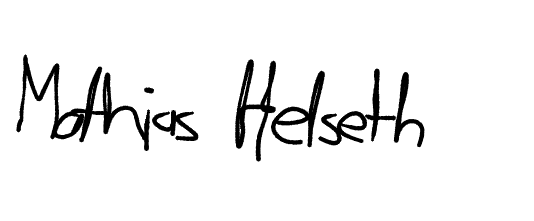
\includegraphics[width=4cm]{signature}

\newpage

%%%%%%%%%%%%%%%%%%%%%%
%%% Table of Contents
\tableofcontents\pdfbookmark[0]{Table of Contents}{toc}\newpage


\newpage
\chapter*{Acknowledgements}
\addcontentsline{toc}{chapter}{Acknowledgements}

\par{I wish to acknowledge and express my gratitude towards the help and guidance provided by my supervisor, Prof. Darren Hurley-Smith at Royal Holloway, University of London. The immense importance of his knowledge and direction that he provided me, greatly benefited this project and report. I would like to thank the School of Engineering, Physical and Mathematical Sciences, Department of Computer Science and Royal Holloway, University of London for the opportunity to write this paper.}

\par{I would also like to thank my family and friends for the support and encouragement through writing this paper during the pandemic. A special thanks to my friend Thomas for providing me snacks and being eminently supportive with his ideas and inputs throughout writing this dissertation. Without his and their advocacy, this would have been an appreciable amount tougher to research and write.}

%%%%%%%%%%%%%%%%%%%%%%
%%% Project Spec or Introduction
\chapter*{Introduction}
\addcontentsline{toc}{chapter}{Introduction}

\section*{Aims}
\addcontentsline{toc}{section}{Aims}
\begin{itemize}
	\item{Exploring how Random Number Generators (RNGs), particularly True RNGs, can be vulnerable in the supply chain against attacks targeting critical security infrastructure.}
	\item{Researching remediation strategies against supply chain attacks.}
	\item{Examining test data from various different RNG statistical test suites, and try to understand their output.}
	\item{Develop a program that implements different test suites in order to (in a user-friendly way) check for structural bias in RNGs.}
\end{itemize}

\section*{Background}
\addcontentsline{toc}{section}{Background}

\par{Random Number Generators (RNGs) are used in various different applications e.g. authentication protocols, cryptographic algorithms and key-exchange protocols. Some of these applications needs to be cryptographically secure by design, and therefore implements a RNG to provide this additional security layer of securing the Confidentiality, Integrity and Availability (CIA) of the system architecture.}

\par{As stated by researcher Tony Gee at the UK based cybersecurity event '44CON' - ``Authentication is not authorization''\cite{Gee:2019}. As this remains true for multiple security applications. Authentication protocols in IoT devices therefore require RNGs to provide a secure layer to authenticate and authorise users between IoT platforms\cite{Cabuk:2017}. There are also examples for the other aforementioned applications that utilises RNGs to provide and achieve cryptographic security. In key-exchange protocols, like Diffie-Hellman, we can apply the power of a RNG to generate secret keys\cite{Mogos:2016}. For cryptographic algorithms, such as SHA-256, RNGs themselves can be enhanced through post-processing the outputs of the RNG with SHA-256\cite{Loza:2015}. We can also use RNGs to create secure keys for use in cryptographic algorithms.}

\par{In the following quote by Vassilev et al.\cite{Vassilev:2014}, the gravity of secure and unbiased randomness through a regularly re-seeded entropy pool is highlighted ``True randomness can't be left to chance. Adopting improved entropy sources that feed into good deterministic random bit generators, together with rigorous estimation of available entropy, will help achieve the guarantees promised by cryptography to protect sensitive information.''. The correct implementations of these RNGs are essential to provide a secure layer. Poorly implemented RNGs may cause implausible implications to the system. An example is non-intentional external bias.}

\par{Statistical tests of randomness can help identify the generators ability (or incapability) of generating random behaviour through analysis of the RNGs output stream. Different batteries of tests exists to perform such analysis, e.g. NIST SP 800-22/800-90b, Dieharder, TestU01 and - although deprecated - FIPS 140-2. The latter is to be followed by FIPS 140-3.}

\par{Despite deprecated and followed by a newer standard, FIPS 140-2 is still in use. Manufacturers and resellers are still labelling their RNGs with FIPS 140-2 certifications and they are still popular in use as lightweight self-tests of Hardware RNGs (HRNG). However, recent research of the tests provided in FIPS 140-2 have shown that they are not capable of identifying tampering of structural bias concealed in the RNG output stream\cite{Smith:2020}. Concealment and implementation of such bias may occur in the supply chain. Unreliable logistics and fraudulent resellers may increase the risk of structural implemented bias. Therefore, we may need proposals of ways to mitigate or completely eradicate these potential risks.}

\par{In a citation from Hurley-Smith et al.\cite{Smith:2020} we learn about the importance of RNGs being secure in the supply chain to alleviate trojanised implications. ``As one of the most fundamental building blocks of any modern crypto-system, RNGs must be trustworthy, unbiased and unpredictable.''. Having a RNG that is secure-by-design, with limited ways of implementing undetectable adversarial bias, combined with a self-test system for the end-user to perform, may lead us in the right direction to protect such a crypto-system.}

\par{Randomness is the key for all secure and non-predictable RNGs. This statement might be obvious, but it can be hard to actually obtain true randomness. A deterministic random number generator, also called a Pseudo-RNG will produce its randomness from a predictable entropy pool. A pool that is enhanced through algorithms and in some cases user-input, we call these entropy sources. We are not able to fill such an algorithmic entropy pool without it being fed with some sort of predictable input. This means that such an RNG would not be fed truly random entropy, leading to non-truly random output sequences in theory.}

\par{As discussed by James M. Rubin\cite{Rubin:2011}, computers are deterministic. They are not able to distinguish or create randomness by nature. They have no conception of what randomness is. These deterministic algorithms that are used to generate what we may know as 'random' in computer games etc., may not be usable in cryptographic applications as computer algorithms are not able to generate randomness. If you are aware of the seed and the algorithm used to generate 'random' numbers. You can predict the output of the generator at any point in time. This makes Pseudo-RNGs unsafe for use in cryptographic applications.}

\par{In a TRNG or a HRNG we employ a physical source for our entropy that is able to generate output that is non-deterministic and not at all predictable. In some cases (which will be explored later in this report.) we benefit from processes, such as emission of radioactivity and noise generated from natural random events to fill our entropy pool. These are not based on a cryptographic algorithm, and it does not require any seed value to produce an output stream.}

\par{Looking at the simple above descriptions, we can differentiate the differences between a PRNG and a TRNG and why we will be focusing on TRNGs and their supply chain in this project. TRNGs are meant to be secure-by-design as they have a physical truly-random event-driven entropy source. However, as seen in earlier in this section. Trusting the supply chain of these RNGs is not feasible. They can be manipulated in the interest of an adversary, and we therefore need to be able to protect them. Especially after it has reached its final destination in this chain. The end-user.}

\par{The objective in this report will be to identify likely threat vectors in the supply chain of TRNGS and comment on the efficacy of statistical tests of randomness performed by the end-user of a TRNG, in order to verify the integrity of the certifications stated by the manufacturers. We defined a PRNG and a TRNG in simple terms above, but it highlights that a TRNG in theory is more secure than a PRNG, due to its entropy sources. The hypothesis of this report, is that the supply chain of TRNGs is vulnerable, and that the integrity of certifications from the manufacturer may be voided in the transportation or reselling process. Finding a way of implementing a user-friendly lightweight statistical test of randomness suite for the end-user, may mitigate the potential use of a compromised TRNG in a system ought to be secure, through alerting the end-user of probable adversarial bias.}


%%%%%%%%%%%%%%%%%%%%%%
%%% Project Specification
\chapter*{Project Specification}
\addcontentsline{toc}{chapter}{Project Specification}
\section*{Feature Specification}
\addcontentsline{toc}{section}{Feature Specification}

\par{In this paper, a user-friendly program for testing Random Number Generators (RNGs) will be developed and tested on both True Random Number Generators and Pseudo Random Number Generators. The program should be able to let the user know whether or not the RNG in question is considered safe to use in environments one would want to be secure. This could be both for company or individual use. The use of known statistical tests of randomness will be used in order to determine this specification.}

\par{The current problem with RNG testing is that it can be both tedious and costly, especially for a company or people that wants to test their RNG for personal use as well. The process can be complicated for individuals who are not familiar with the statistical tests, and therefore the testing of these RNGs can be neglected. Having a friendly graphical user interface with easy test output can help deliver a quick and easy testing tool for these individuals and companies.}

\par{The importance of testing these RNGs is invaluable. Adversaries can implement bias into these RNGs as we will se later on, which can seem random to the human eye, but greatly impact the output of them. One type of bias is structural bias. This can be implemented in the output stream from the RNG and help an adversary infiltrate a system by revealing e.g. secret keys in a cryptographic system. Due to this importance, having a simple way of testing these RNGs is necessary.}

\par{There are multiple batteries of statistical tests that can be used in order to test a RNG, but to keep this paper and report concise; 1-2 test suites will be selected. An approximation of three minutes maximum testing time is preferable. This is so that the user can feel comfortable with the test results (Some level of exhaustive testing), but still be time efficient.}

\par{The program will accompany a progress bar to show the user the progress that has been made. This is to help the user with time management. If the user can see the progress and know where in the testing process they are, it is possible that they will keep using the program. If the program did not have a progress bar, the user could be left uncertain whether or not the program is functioning. Especially since the loading time of the tests performed in this paper will be up to 3 minutes long.}

\par{It is important that the result of the tests shows up as a binary yes/no to the user. As the program is meant to eliminate the exhausting steps to use statistical testing in the first place. The output data of statistical tests can be assumed to be hard for a user to interpret, especially if the result is coming back has not passed. We will learn about the use of p-values as a mean of determining if a test has passed or not, in this report. However, as we want the program to be simple, a binary output is sufficient.}

\section*{Technology Choices}
\addcontentsline{toc}{section}{Technology Choices}

\subsubsection*{TestU01}
\par{For the actual testing of Random Number Generators through statistical tests of randomness, a library named TestU01 will be used. The library is written in C, and to use it, compiling C code is required. The library consists of multiple statistical tests, test batteries and Pseudo-Random generators. This library will be used, because of its multiple integrated test batteries with clear specifications when it comes to input size and format needed to test a generator. TestU01 can be hard to understand and implement for a new user. Therefore, a friendly graphical user interface will accompany it, within an easy-to.install package.}

\subsubsection*{Python and Tkinter}
\par{Python has been used as the main programming language for this program. The simplicity that can be achieved with python, and how easy it is to combine with the C language's standard output (stdout) is why I chose this. The use of the library Tkinter was necessary to generate the Graphical User Interface (GUI). It is flexible and efficient for use with the implementations that I have created in C from TestU01. I am able to let the user navigate through my program, and at any point of time know the progress of the testing using a progressbar module inside Tkinter.}

\par{While Tkinter is a great GUI module for Python, and easy to compile into a neat package. There are other alternatives that also were considered, but that I did not end up with in the end. For example, libraries such as PyQT5, PySide and wxPython were all considered in the beginning, but I chose to go for Tkinter, because it is widget-based and has a simple documentation which goes straight to the point for each widget.}

\par{Also, a reason for choosing Tkinter was because it was seamless to implement threading for the progressbar. Tkinter uses threading to provide some of its support for multiple window pop-ups. Which could have been obstructing my intentions of running threads in the background using the 'threading' module. However, with Tkinter this works smoothly. My progressbar needs to be running in its own process while the tests are running, and it is also nice to have the tests run in its separate process. This is to eliminate the chance of the program not letting the user exit, or interact with the program as it would simply freeze during the execution of the tests.}

\par{The threading process in Tkinter is running a mainloop. This loop is its own thread, and all the code that is running inside tkinter will be running on this thread. Therefore, exiting the program, or performing other tasks will not be possible without having multiple threads open. That is why the threading module is used in this particular case.}

\subsubsection{Makefile}
\par{To ensure that the user will be able to run the program, and have the necessary libraries installed when trying to do so. A Makefile is used. The Makefile is a simple file with executable commands that ensures that the user has the sufficient libraries in order to successfully run the program without any compilation errors. The user of the program simply needs to install make on their system, and run it through the command 'make' in order to install the appropriate packages. This is good for the purpose of this report. However, if this were to be a released program to the public, the use of a binary executable file programmed in C would be more efficient probably, rather than a python file that needs to be run manually.}

\par{During the development of the program, I realised there was a bug in one of the programs that was needed to run output data out of a particular TRNG. I needed to replace this file with a fix. Since the GitHub repository for this code was not well-structured, and where containing zip archives for the binaries. I had to create the file in a cloned repository and replace the file manually through the terminal. A Makefile made it simple to clone their repository and provide the new fix seamlessly into a local repository on the user's end.}

%%%%%%%%%%%%%%%%%%%%%%
%%% Literature review
\chapter*{Literature Review}
\addcontentsline{toc}{chapter}{Literature Review}

\par{This chapter is dedicated to demonstrate my insight into the project through the research publications I have read so far. }

\par{While there has been a significant amount of research done on the different statistical test suites and their vulnerabilities, there has been less research dedicated to identifying threat vectors in the supply chain of RNGs and remediation strategies. Therefore, I have focused my project towards this topic. I am interested to see if there has been done research which concludes any of my questions that I raise in my reports. I hope to be able to produce a program in the end of this report to demonstrate the potential efficacy of end-user statistical testing to ensure that the RNG is not biased before it is put in use. It could have been affected in a negative way in the supply chain or after reselling, potentially by an adversary.}

\par{Organisations that might require an RNG on-site are in the countless numbers. Security is nonetheless important, TRNGs can help many organisations and individuals to improve their system and application security. The problem these users can face from the RNGs are the lack of knowledge regarding the infiltration vectors. Therefore in this review and in the report, it is assumed that we are needed to inform a new user of an RNG whether or not the specific device can be trusted. Our approach might not mitigate all potential attack scenarios, but it might help create a cost-effective and time efficient combined suite.}

\par{Who should be responsible for the integrity of these devices? Probably the manufacturer (especially at the point-of-manufacturing), however, after it has left the manufacturing facilities, they can't monitor the integrity and it is left to the user to ensure that this attribute of security withstands. Manufacturers can claim their product is tamper-resistant, but a RNGs internal entropy source for the actual generation of randomness in the entropy pool may get damaged. How can we ensure that this entropy pool is fresh and renewed with a reliable source? Here, an approach to detect anomalies found in both attacks and entropy source degeneration would be feasible.} 

\par{In my \nameref{SupplyChainAttacksReport} report, I have found that there could be introduced several different attacks towards TRNGs while they are circulating in the supply chain. In the report I raise several questions as to why the RNGs can't be trusted when received to the end-customer and why we safely can't assume their integrity even when in use. The manufacturer can label their TRNGs with certifications from different test suites such as FIPS 140-2. However, after it has left the manufacturer, we can't rely on the manufacturers claims of passing these certifications anymore. Can we introduce a self-testing system for the user?}

\par{The main concern for researchers that have been analysing different statistical test suites, seems to be that the tests fail to discover underlying bias from potential adversaries. This could be a substantial threat to companies and individuals adopting these RNGs into their systems to generate e.g. cryptographic tokens. Performing statistical tests of randomness is not especially hard, and can be done by most individuals. The problem occurs when time and cost is a constraint. A company that receives a couple of RNGs to be used in their applications, may not have the time to perform huge and thorough statistical tests on all these devices. They might not be interested in paying a third-party security firm to perform testing on these devices as it would be a huge short-term investment for them. Having an internal audit of the security of the RNG may be a solution, but it will take time and educating the employees will be necessary.}

\par{``In every organization, whenever an investment has to be made, everybody is concerned about the return which the organization will be getting from that investment. Every investment has to be justified from the point of view of return. Investments made in cyber security are never preferred by the organizations as they do not give any return. Return on Investments made in Cyber security is not measured in terms of profits and gains, but rather in terms of prevented losses.''\cite{Kesswani:2015} As companies reluctantly want to spend money on cyber security and data protection, it can have negative long term effects. RNGs can provide an important security layer in a system. Therefore, I believe it is important to look at alternative cost and time beneficial methods to perform these statistical tests of randomness at the point where the TRNG is supposed to be used.}

\par{The proposal of such a system would be based on the research already done by researchers on TRNGs and their vulnerabilities to be affected by structural bias. Such as in \cite{Smith:2020} where Hurley-Smith et al. performed statistical tests of randomness on the following \ref{fig:Smith2016_einstein} WEBP image of David Rothman and Albert Einstein, and it passed all the tests in the FIPS 140-2 suite of statistical tests. This led them to the following thoughts ``If an image can be reduced to such a compressed, apparently random state that it can pass statistical tests of randomness, it may be possible to encode such images into the output of PRNGs as a form of information leakage.''\cite{Smith:2020}}

\begin{figure}[h!]
\begin{center}
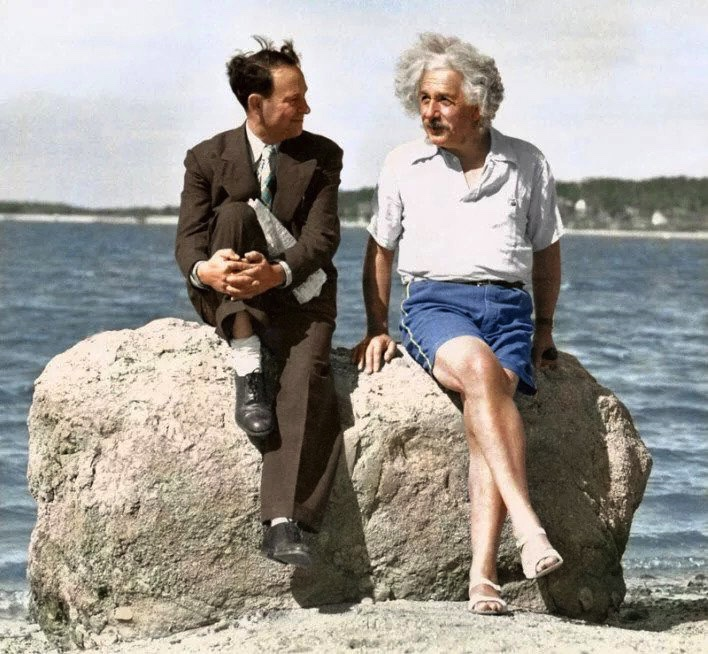
\includegraphics[height=8cm]{Smith2016_einstein}
\caption{This WEBP image passes all tests in the FIPS 140-2 suite\cite{Smith:2020}}
\label{fig:Smith2016_einstein}
\end{center}
\end{figure}

\par{If such a WEBP image can be implemented as a mean of structural bias in a PRNG. What stops it from being hidden inside a TRNG? As some manufacturers might be proud of their FIPS 140-2 certification and label their TRNGs with the passing of all the tests in this suite. Some end-users may not think twice about using this RNG in their system because of this certification. However, as clearly seen in this example we have an insecure RNG that can output non-random sequences affected by the data in a WEBP image.}

\par{In this project there has been reason to particularly look at two different types of RNGs. True Random Number Generators (TRNGs) and Pseudo-Random Number Generators (PRNGs), where my main area of focus has been TRNGs. While there exists another fraction of TRNGs which extends further than the classical ones, namely Quantum Random Number Generators (QRNGs). I have settled with researching the supply chain of TRNGs which derives from physical processes, such as thermal noise and radioactive decay. The reason being that QRNGs would advance the project out-of-scope.}

\par{I have focused on researching existing publications on vulnerabilities against TRNGs in-and-out of the supply chain. To be able to reason about the supply chain and RNGs in greater detail, some tests have been conducted to better understand the underlying factors used in the different batteries of tests found in statistical test suites. For these tests to be conducted, I have been implementing code in Python and C in a UNIX environment to test different TRNGs and also the /urandom and /random PRNG generators found in most UNIX distributions.}

\par{The reading I have been doing for this report has been varied, as I am looking into both RNGs and the their supply chain. Currently, my supervisor's previous work in this field has been very relevant and multiple citations have been made from his work in this report already. The work of Hotoleanu et al. has also contributed to comments I have made in this report. In a research paper from 2010, they found that a hardware implementation of statistical test suites can be of advantage to the user, as it can be faster and more reliable as it is built-in. However, there were some drawbacks of a FPGA implementation, as only 8 out of 14 tests of the NIST SP800-22 suite were suitable to hardware implement in that particular scenario.\cite{Hotoleanu:2010}}

\newpage
\section*{Hardware Random Number Generators}
\addcontentsline{toc}{section}{Hardware Random Number Generators}

\par{Hardware Random Number Generators (HRNGs) benefits from random events from a physical source in order to generate its entropy pool. The output bit-stream of a HRNG will be non-deterministic and independent and identically distributed, which means that the outcome of each bit in the bit-stream has the same probability distribution. Some examples of HRNGs are the ChaosKey by Altus Metrum and TectroLabs TL200. These are available to purchase, and are supported by certifications that we will discuss later on, such as FIPS 140-2 and NIST SP800-22.}

\par{The physical source of randomness in HRNGs can come from various different natural phenomena, such as decay of radioactive materials\cite{Rohe:2003}, thermal noise\cite{Rohe:2003} and atmospheric noise\cite{Jun:1999}. As Stipčević et al.\cite{Stipcevic:2014} states,``Our assumption has been that random numbers cannot be computed; because digital computers operate deterministically, they cannot produce random numbers", therefore we use random numbers generated from a physical entropy source. Such RNGs are called True RNGs.}

\par{Pseudo-Random Number Generators (PRNGs) on the other hand harvest entropy from software events and cryptographical algorithms. As PRNGs rely purely on software implementations, and its entropy comes from algorithms rather than actual physical and random events, it is deterministic. As Hurley-Smith et al.\cite{Smith:2018} notes, PRNGs are initialised through seed values which rely on entropy, usually from the OS entropy pool. Also, as written in \cite{Gong:2019} ``PRNGs use some initial seeds and deterministic algorithms to produce pseudo-random numbers and can result in high throughput. However, once the seeds are obtained by attacker, all security will be lost. Thus, it is dangerous that using PRNGs produce secret keys.''. These generators are particularly great to use when for instance generating Monte Carlo simulations\cite{Bosque:2019} or other simulation/modelling scenarios, but due to the exposure mentioned above we do not use them for much else.}

\par{HRNGs can also be used as a hybrid generator in conjunction with PRNGs. In this case the HRNG is used as a seed generator for the PRNG. Using the HRNG and a PRNG together as a hybrid solution will create a Cryptographically Secure RNG (CSRNG), which is a subset of PRNGs. Some of these are considered to be very fast, and in many applications, more reliable than simple PRNGs\cite{Bosque:2019}. A CSPRNG needs to follow some requirements in order for it to use its initials - cryptographically secure. It needs to provide forward-secrecy, a big key space and also a highly-sensitive key values. Having these essentials, we find in \cite{Bosque:2019} ``These requirements are set to assure that, unless the full key is known, it is not possible to predict the output values or extract any kind of information about them. A PRNG that is suitable for these applications is often called a Cryptographically Secure Random Number Generator (CSPRNG).''}

\par{We can implement whitening functions, or so-called post-processing methods, to CSRNGs to remove non-random attributes from the output stream of such a RNG\cite{Holleman:2008}. A whitening function is an algorithmic strategical method to clean up the output of a raw TRNG. Examples of such functions are Von Neumann or XOR-operations over the raw bit-stream output. As stated here \cite{Gong:2019} ``While some entropy sources are claimed to directly generate enough random bit sequences, most TRNGs produce imperfect random bits without post-processing. To avoid this problem, TRNGs should include a well-designed post-processing, which can reduce statistical flaws and provide prediction resistance.'' we use these whitening functions - or as called here - post processing to get rid of these ``imperfect random bits'.'}

\par{Are we able to differentiate the output of a TRNG, PRNG and a CSRNG? Probably not, as it often looks like absolute gibberish, which is the point. Why does it then matter if we have a physical and natural noisy entropy source, instead of a computed algorithm seeded with user input? For computer games, statistical analysis, simulations, emulations etc., a PRNG and a CSRNG would probably do just fine. Supposing we would like to add some security and unpredictability into this. A TRNG would be very beneficial. Therefore, we can adjudge that for different applications and security needs, applies appropriate RNGs. Here is an example from the 5G industry \cite{Lee:2018}, ``In particular, proposed TRNG can provide more secure communication because the TRNG can generate a random value and utilize it as a key for each entity, for example a base band and a station, in 5G network.''}

\par{In cryptography, the use of unbiased, unpredictable and entropically rich RNGs are essential to prevent potential adversaries from gaining insight or part-control of a system. As \cite{Thamrin:2008} notes ``Since all security protocols rely on unpredictability, RNGs for crypto applications must meet stringent requirements.'' we can't be permissive of what sources we use for our entropy, and we can neither rely on certifications that may advocate for a specific vendor. For our RNGs we simply have to be able to trust them at point-of-use. Trojanised and biased output from a RNG may lead to catastrophical consequences where adapted. A proposal for an enhanced, but lightweight testing suite may help out. However, there are most likely only mitigations to be made, no definitive solutions to the problem of trojanised RNG output through structural bias.}

\par{The reason for PRNGs not being able to provide the same level of security as a RNG - based on hardware implemented entropy sources, can be demonstrated. In a PRNG, the entropy pool can fill up or stop being refreshed with new input data. This makes PRNGs less cryptographically secure. Especially in blocking mode, where the PRNG will stop outputting numbers if the entropy pool lacks input data. As well as the problem with PRNGs where, if you know the seed, you can generate or predict new numbers. If we make an assumption that we have the entropy pool in one PRNG fill up with user input (clicks, mouse movement and keystrokes). This can at any point stop being fed new input, and therefore the generator will have to take its inputs from the same entropy pool (assuming we are using a PRNG that is not in blocking mode e.g. dev/urandom). This can lead to the generator outputting sequences or simply repeating the same patterns, which is insecure for many reasons. Including the ones mentioned. In time-effective applications, a non-blocking PRNG would likely be preferable, even though the security could be affected.}

\par{As we can see in Figure \ref{fig:TableA} by Vuillemin et al. \cite{Vuillemin:2012} in the first output table, the amount of entropy gathered from user input is substantial in PRNGs. The problem is that we can in fact run out of this user generated entropy. At startup or system reset, the Linux kernel does need at least 192 bits\cite{Mowery:2013} of external (e.g. user-generated) entropy before it starts employing this entropy to create its own system entropy.}

\begin{figure}[h!]
\begin{center}
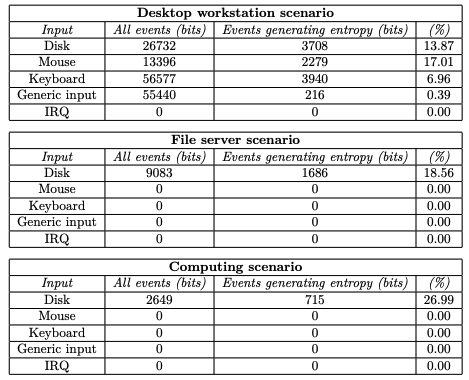
\includegraphics[height=8cm]{TableA}
\caption{Proportion of input events that generate entropy\cite{Vuillemin:2012} in a Linux RNG entropy pool.}
\label{fig:TableA}
\end{center}
\end{figure}

\par{In some cases a system may generate 'bad' entropy, through e.g. attacks or bad implementations of the RNG. As seen stated here\cite{Bellare:2009}:  ``Cryptography ubiquitously assumes that parties have access to sufficiently good randomness. In practice this assumption is often violated. This can happen because of faulty implementations, side-channel attacks, system resets or for a variety of other reasons.'', In 2008, the OpenSSL\cite{Yilek:2009} package on some Debian systems were found to have a vulnerability with its entropy pool, which caused it to lack enough entropy to keep its SSH and SSL services secure. Leading to private/public keys becoming predictable for potential adversaries.}

\par{As we have previously discussed, respective TRNGs have different ways of gathering a constant fresh source of entropy. These are physical and natural events processed at an unpredictable rate. This physical noise is produced, captured and in the background, a whitening function, helps clear out the bad input. The most commonly used entropic sources that I have found in the TRNG public market are among others, decay of radioactive materials\cite{Rohe:2003}, thermal noise\cite{Rohe:2003} and atmospheric noise\cite{Jun:1999}. These sources of entropy allows the TRNG to produce secure and unpredictable random numbers to be used in various applications.}

\par{Currently, on the market there are a number of different vendors selling their TRNGs\footnote{\url{https://www.aliexpress.com/af/TRNG-noise.html} and \url{https://www.amazon.com/TrueRNG-V3-Hardware-Random-Generator/dp/B01KR2JHTA}}, both by individuals and by corporations manufacturing them. The majority of these TRNGs are marketed as being able to pass most of the top industry standard statistical tests, such as Dieharder and FIPS 140-2 just to mention some of them. This seems to be one of their main selling point, in addition to their output speed. Now, can we trust these statements without actually testing this ourselves? These devices are trusted by users at point-of-use, probably without many of them testing them through exhausting statistical tests of randomness. There might be a good reason for this. Exactly as the last sentence stated. The tests are exhaustive. Especially for individuals. Another reason to make them lightweight and easier to understand for the end-user.}

\par{The industry standard test suites are usually said to be performed by the manufacturer, which provides the results to the end-user. How can we however know that the RNGs have been altered after the tests? As discussed earlier in the literature review, the entropy source could have been exposed to external bias, which could have been not picked up. These are vulnerabilities that can be found in most TRNGs purchased online or even just in general.}

\par{PRNGs lack robustness in many applications and are posed as more vulnerable to injection of trojanising input. Let it be malware, other invasive means of intrusion or not properly seeded PRNGs. Looking into the dev/urandom and dev/random PRNG that is delivered in most UNIX distributions. Their entropy pool is filled with user input, system events and disk noise\cite{Vuillemin:2012}. Even though we make harsh claims about PRNGs, they can be used for cryptographic applications. In the UNIX distributions, urandom is often preferred\cite{Huhn:2014} due to its non-blocking capabilities over the blocking in random. Blocking means that the RNG halts the number outputting if it is not provided with enough entropy at the point of generation. Using urandom when it is properly seeded, should be more than suitable for most applications\cite{Huhn:2014}.}

\par{We have looked into different RNGs, especially of the type PRNG. Now, since this project is focusing on the TRNG market and its vulnerabilities in and out of the supply chain. I have conducted a market analysis of the available TRNGs. From the table below, we can see some of the TRNGs available to purchase and which technology they apply to produce their randomness entropy. Also known as their entropy source. I chose to collect the first 5 TRNGs that I could find crawling the web for TRNGs, just to give a general image of price, claims and use of entropy.}

\begin{tabular}{ |p{4cm}||p{4cm}|p{3cm}|p{3cm}|  }
 \hline
 \multicolumn{4}{|c|}{\textbf{\textit{Market research of available TRNGS}}} \\
 \hline
 \textbf{TRNG}& \textbf{Entropy Source} & \textbf{Tests passed} & \textbf{Price}\\
 \hline
 Infinite Noise TRNG  & Thermal Noise (MEM) & FIPS & 35 dollars\\ 
 \hline
 Araneus Alea II & Amplified semiconductor white noise & NIST / Diehard & 99 euros \\
 \hline
 BitBabbler White & Analogue Noise & FIPS 140-2 / NIST SP800-22 / Dieharder / Ent / TestU01 / AIS-31 / Etc...& 150 dollars \\
 \hline
 Tectrolabs AlphaRNG & Electrical diode noise & NIST / Dieharder / Rngtest / IID / Ent & 499 dollars \\
 \hline
 Quantis QRNG PCIe and USB (Legacy) & Quantum Noise & NIST SP800-22 / NIST SP800-9b / Dieharder & 1335 euros\\
 \hline
\end{tabular}

\par{As we can see from the above table, TRNGs comes in various types, and they can be both cheap or very expensive. One interesting thing to note, from the 5 listed TRNGs, we can see a correlation from price to the altitude of tests passed (claimed by the manufacturer). Maybe this is because the manufacturer do not want to make bold statements, that can later be undermined the power of and be used against the TRNG or the specific manufacturer. i would say this is a good thing, as it certainly makes it more relevant to perform own tests.}

\par{However, we do see that BitBabbler make bold statements regarding number of tests passed. When accessing their website\footnote{http://www.bitbabbler.org/what.html}, they claim to pass a number of additional tests as well (More than the ones listed in my market research table above). What is concerning about this exact TRNG vendor and its claims, is that for e.g. TestU01, they consider it to be of such magnitude (ref: the test result data from TestU01) that they exclude the test results, and conclude that a 200 page document is too long. This is concerning as it does not show a sophisticated understanding or systematic way of testing from their end. Especially when they claim that it passes all these other test suites as well.}

\par{The consequences of a TRNG being validated for all these tests without proper corroboration of the results, is that it will become trusted by the end-user when it is in fact not secure. In most cases, vendors will provide test details and logs from the actual test suite run. This is also a great way of earning the users trust, but we can still not take it for granted that we can depend on these test results. Especially when the TRNG has been in the supply chain and eventually ended up in the hands of the user, after being sent through multiple vulnerable instances.}

\par{When using TRNGs in cryptographic applications, we may want to set and follow some guidelines in order to ensure that we are operating it securely. This is especially true for TRNGs ending up in corporations or firms where security is a high priority. Following the principles of the evaluation document of AIS-31\cite{BSI:2013}. A test suite and standard from the Bundesamt für Sicherheit in der Informationstechnik (BSI) or in English: The German Federal Office for Information Security. We can extract some guidelines that we can set for our use of TRNGs in environments we want to keep secure.}

\subsubsection*{Loosely extracted Guidelines from BSI AIS-31\cite{BSI:2013}:}
\begin{itemize}
    \item We must be allowed access to the structure of the TRNG (How it is built and how it generates its entropy)
    \item Post-processing of the TRNG output through a PRNG/CSPRNG whitening function should be a requirement in all cases.
    \item We must be able to test the RNG ourselves to ensure that it meets with our own standards if that is more preferable than trusting certifications gathered from the manufacturer
\end{itemize}

\par{These guidelines are just a personal excerpt and interpretation from the standard documentation of AIS-31. The documentation involves an evaluation scheme for auditing Random Number Generators in environments where it needs to produce secure numbers. This can be especially important in government, industrial or military applications. The NIST SP800 standards and testing suites are yet another example of documentation that involves evaluating RNGs. PRNGs can also be evaluated through such a scheme, but the use in TRNGs is often useful to determine if it has an underlying trojanised bias. To not leave out details, PRNGs can experience malware or other trojanising bias as well, but this would leave us out of scope for this project report, as PRNGs can in some cases suffer from some very much different adversarial attacks.\cite{Cornejo:2014}}

\par{If PRNGs are thought to be less secure than HRNGs, why are they in use? Well, some applications does not require the security layers that a TRNG can provide us and only used for convenient systems. An example of this is Spotify and how they used to shuffle their playlists back in pre-2014\cite{Polacek:2014}. Spotify users complained that their playlists were not shuffled randomly and that songs from the same artists would reappear multiple times in a 'random shuffle sequence'. The Spotify Engineering team speculated why this was the case, as they had followed the users request and implemented a random shuffling algorithm (Fisher-Yates shuffle\cite{Toutenburg:1971}). However, the problem with this implementation is that it was 'too' random for the users. Music from the same albums and artists would also sometimes cluster. Following this, Spotify decided to implement a dithering algorithm on top of this, to eliminate annoying patterns in the sequence\cite{Polacek:2014}.}

\par{When we perform statistical tests of randomness on TRNGs, they can tell us more about the underlying characteristics, other than the rather obvious, the entropy source. We can more easily determine if a generator should be used for a specific purpose or whether we should abandon or control some of the risks associated with the device. e.g. set up device controlling and monitor its output while in use to look for inconsistencies or abnormalities.}

\par{As discussed, there are multiple test suites available. When we later on will be looking into methods to test these RNGs with statistical test batteries, we will be using a combination of some well-known test suites. We know that some test suites are not very good at picking up structural bias from a large set of input data. Such as the FIPS 140-2 set of tests\cite{NIST:2019}. Even though this test suite was (now deprecated and no longer recommended for use) a US/Canadian federal standard, it has now started to loose its recognition. It will be replaced by FIPS 140-3\cite{NIST:2019}. The FIPS 140-2 tests were meant to disclose adversarial bias, it did however in some cases fail to do so. FIPS 140-3 will advocate for self-testing and other methods of mitigating threat vectors implemented in the RNGs. } 

\par{FIPS 140-3 has in its transitional effort from FIPS 140-2 put in some guidelines it will try to follow, which is in contrast to FIPS 140-2 more aimed towards early prevention and also helping end-users test their devices in advance of using them at the point-of-use. As they state about their efforts in \cite{NIST2:2019}``These areas include cryptographic module specification; cryptographic module interfaces; roles, services, and authentication; software/firmware security; operating environment; physical security; non-invasive security; sensitive security parameter management; self-tests; life-cycle assurance; and mitigation of other attacks''.}

\par{Some other tests suites include, Diehard, Dieharder, Ent, TestU01, AIS-31 and NIST SP 800-22/800-90b. These are popular tests to use, but most of them (except NIST and AIS) are made from a non-governmental standard association. This does not directly imply a negative effect towards the test suites. It might actually be a positive collection of tests as it may lead to more open source information regarding the methods and ways of testing. Which again makes it easier to incorporate in user-friendly testing applications. However, NIST (which also develops the FIPS tests) publishes documents describing the use of the standard in great detail.}

\par{These test suites do have a problem that they share between them. Namely a common standard issue, where the test suites are very similar in many ways. Incorporating the same tests. As highlighted by Hurley-Smith et al. \cite{Smith:2020}, ``AIS-31 procedure A still uses FIPS 140-2, and manufacturers continue to use FIPS 140-2 test results as a form of quality assurance. The reliability any verification process implementing these tests must be considered suspect. This work, indirectly, also highlights the large degree of correlation between the different tests in popular randomness test suites (namely FIPS 140-2 and AIS-31). This is a well-known problem [31], [32] that has not been tackled yet. This intra- battery test correlation makes it easier to design adversarial generators capable of bypassing all the randomness tests in a given set of standards.''}

\par{As we have seen, Random Number Generation through a physical and natural event as entropy source, is possibly the best and most secure way of generating these random numbers. The reasons are many, but mostly that the numbers are not generated through algorithms, but noise found in nature or analogue processes and are therefore non-deterministic as a result. As the bits or numbers in the sequences generated by the hardware generators are not related to one another, and they are Independently and Identically distributed (IID), we can say that they provide forward-secrecy. Also backwards-secrecy. This is a major security benefit for making sure that if an adversary gains access to the output, they would not be able to predict future or previous bits/numbers.}

\par{Now, the new term IID has come to our attention. It can be detailed in simplistic terms without excessively perplexing it. We usually speak of IID in probability. The probability of some outcome in our RNG should be identically distributed, which means that every combination of any outcome should be the same. The RNG should also output numbers that are independent of each other, meaning that the next number should have no connection with the last number, forward and backwards secrecy.}

\par{Even though we say a RNG is IID, non-deterministic and is provided with forward/backward-secrecy, we do not know whether or not to trust the output, as the adversaries may implement bias or unintentional bias from surroundings/deprecation of the RNG. Therefore it is important to stress the fact that statistical tests (especially self-testing) of randomness is necessary and critical in many applications that is devoted to cryptographically secure systems. This remains true for private use as well, while companies can potentially suffer greater damage if these devices are not routinely checked for structural bias through appropriate testing.}

\newpage
\section*{Supply Chain Attacks} 
\label{SupplyChainAttacksReport}
\addcontentsline{toc}{section}{Supply Chain Attacks}

\par{Currently, Random Number Generator (RNG) manufacturers continuously use the statistical tests of randomness found in standards such as FIPS 140-2 to prove that their RNG is cryptographically secure. Even though this particular standard for statistical tests is now starting to become deprecated \cite{NIST:2019}, it is still widely used manufacturers to prove that their RNGs are producing output which can be used in cryptographical applications. How can we know that the claims of the manufacturer stand true at the point it is handed to the end-customer and it has been through the supply chain?}

\par{If we assume three phases of the process of distributing Hardware RNGs (HRNGs). Just to provide an example of the level of trust signed by the end-customer to the RNG manufacturers. The manufacturing phase, the supply chain and then leaving the supply chain to the end-user or organisation. In these phases, we can assume that there are different vulnerabilities that can be introduced to the RNG in circulation. Either by adversaries or through unintentional external/internal bias.}

\par{Taking precautions before applying these RNGs in any secure environment is important. We probably can't prevent adversaries from entering the supply chain, but we can take action before it is to be used for cryptographic applications.  If the statistical tests are to be trusted, they should be able to detect adversarial structural bias, because it can have such great damage effect on a system. As Hurley-Smith et al. \cite{Smith:2020} states in their journal on the lightness of FIPS 140-2, “Our research shows that FIPS 140-2 cannot identify adversarial biases effectively, even very primitive ones.”. This can lead us to think that this commonly used statistical testing suite, can’t be trusted for use in testing the integrity of an RNG after it has been manufactured.}

\par{For statistical testing of randomness, there are generally a series of tests being performed on huge n-bit-blocks from an output stream. These tests look for particular distinctive characteristics usually found in random sequences. In the NIST SP800-22 and FIPS 140-2 batteries of tests for example, we find similar \cite{Smith:2020}\cite{Rukhin:2010} tests being used for general testing, such as the monobit test, where we test to see if the number of ones and zeroes in a bit-block sequence are approximately the same as in a truly random sequence. Here we are again looking for an Identically and independently Distributed (IID) sequence of numbers.}

\par{As stated by Bill Phelps, Commercial Lead in Booz Allen Consulting \cite{Phelps:2019}, increasing the visibility into the supply chain, a good relationship with the suppliers and planning remediation strategies against breaches can help the manufacturer mitigate supply chain attacks. These attacks could even happen physically towards the RNG creating external bias to the RNGs entropy source. Such as with thermal noise RNGs where noise-based attacks can be executed to create structural bias in the RNG \cite{Brown:2020}.}

\par{An adversary may be interested in implementing bias to the RNG, while still making sure that it will be able to pass the most common batteries of statistical tests. Presumably at any point should the tests pass, and especially important for the adversary that it passes when the end-user tests it. However, we can’t safely assume that the customer will be able to perform these software tests on their own, as it may require some technical knowledge of RNGs at this point in time. They can be time consuming to perform and require some background information of the statistical tests in order to understand the results. By implementing a low-cost on-chip hardware layer of lightweight statistical tests that may allow for trivial steps to be performed by the consumer, we may be able to mitigate some of the adversarial biased RNGs entering the systems.}

\par{On-chip hardware statistical tests could be an addition, but maybe not alternative, to the software-based statistical test batteries that exist today. As Hoţoleanu et al. \cite{Hotoleanu:2010} notes, during their experiment implementing the NIST SP800-22 statistical tests onto a FPGA board. They found that only 8 of the 14 tests\footnote{14 out of the 16 total tests in the NIST SP800-22 were recommended by NIST at the time of their experiment\cite{Hotoleanu:2010}} were suitable for lightweight hardware use. Yang\cite{Yang:2016} also found similar results with a FPGA implementation of NIST tests.}

\par{Having these hardware implemented tests we could introduce new solutions to deal with adversarial analysis of the RNG. By introducing a decontamination protocol for the end-customer, where the RNG is to be placed under a strict test regime during its first entry under new hands. This could help mitigate unexpected/unwanted behaviour in the RNGs by finding potential leaks in the design through statistical testing. This may however not be to any help if the adversarial input bias is well designed, lacks flaws and/or are able to pass the statistical tests.}

\par{In having hardware implemented tests, we could create an isolated environment to run tests in. It would not be affected by anything other than the actual RNG. This is good, but as noted by \cite{Hotoleanu:2010} not all tests are suitable to be hardware implemented. Therefore it could be proposable to invest in developing tests that are designed to be performed on board. This may be beneficial in the long run, as supply chain attacks could more easily be discovered if the actual test suite was hardware implemented, allowing the user to simply test the RNG with on-board logic communicating directly with its entropy pool.}

\par{As mentioned in \cite{Becker:2020}, ``In recent years, hardware Trojans have drawn the attention of governments and industry as well as the scientific community. One of the main concerns is that integrated circuits, e.g., for military or critical-infrastructure applications, could be maliciously manipulated during the manufacturing process, which often takes place abroad.'' We have an increasing amount of uncertainty regarding future attack access points, but working proactively can ensure that we are better prepared. Luckily, we are not aware of any major hardware trojans being implemented in RNGs yet, neither in other electrical circuits. ``However, since there have been no reported hardware Trojans in practice yet, little is known about how such a Trojan would look like, and how difficult it would be in practice to implement one'\cite{Becker:2020}'}

\par{Looking at the experiments conducted by Hotoleanu et al.\cite{Hotoleanu:2010} and Yang\cite{Yang:2016} to implement statistical tests in hardware. We have some tests that can be implemented, and some that can't be, due to limitations. Generating a protocol to separate which tests that can be implemented in hardware and which that needs to be implemented in software. it could be possible to define a maximum number of tests needed to execute a given test suite appropriately (or define a new test suite) in hardware. This could further help us find faster and more reliable testing mechanisms for the end-user.}

\par{So, we should assume that no RNG that has entered the supply chain is safe to use. Not only adversaries are a threat as we have discussed, also the entropy. Gong et al. \cite{Gong:2019} clearly discusses the importance of post-processing of the TRNGs. ``While some entropy sources are claimed to directly generate enough random bit sequences, most TRNGs produce imperfect random bits without post-processing. To avoid this problem, TRNGs should include a well-designed post-processing, which can reduce statistical flaws and provide prediction resistance.''. This is important to remember, as it has a huge amount of meaning to the output stream of the RNG.}

\par{Not only are direct adversarial attacks and entropy post-processing sources of confusion for the statistical tests of randomness. Jianxin Xu, at the School of Management at Hangzhou Dianzi University in China recognises some of the developments in the supply chains over the years\cite{Xu:2008}. Not particularly for RNGs, but in general for consumer products and secure devices that may be vulnerable. ``Disruption risk has received increasing attention in the last few years, when it comes to global supply chains, the potential for disruption comes in many packages, from large-scale natural disasters and terrorist attacks to plant manufacturing fires, widespread electrical blackouts, and operational contingencies such as shipping ports too small to handle the flow of goods coming into a country.''}

\par{As he very well notes. There are many other supply chain vulnerabilities, then what we have discussed as of now. Not that this may be too relevant for our TRNGs, but these threats exists as well. High temperatures in a storage room may very well damage a thermal entropy source, the same goes with cold temperatures. As the devices travel to multiple destinations with varying climate, manufacturers should acknowledge that this may very well become an issue. Other external bias scenarios include radioactive input from surroundings, affecting for example TRNGs powered with a geiger counter for collecting its entropy from a radioactive source.}

\par{From the creators of the ChaosKey TRNG, Altus Metrum, they stated during a Debian conference back in 2016 \cite{Garbee:2016} that the ChaosKey 1.0 would be secure against software attacks. As it passively looks for hardware interaction (shorting two pins on the actual hardware chip) to reflash the software image loaded on the board. They do admit that even though it is resilient against pure software attacks, once it leaves their hands, they have no control over the hardware. This again states our important message, that once a RNG is out of the manufacturers hands, we can't guarantee that the manufacturers claims regarding passing different tests still holds. Hence, the use of statistical tests to detect bias that may harm a system is imperative.}


%%%%%%%%%%%%%%%%%%%%%%
%%% Methodology
\chapter*{Methodology}
\addcontentsline{toc}{chapter}{Methodology}

\par{In this chapter we will be going through the methods and theory behind the development of a collection of statistical tests of randomness, that can easily be performed by an end-user to verify that their RNG is feasible to use in a secure environment. Hopefully in a way of self-testing that mitigates some of the threats entering the end-users system, as we saw introduced in the supply chain. We discussed that structural bias and other bias may be harmful to a system meant to be secure. Having a way of isolating the tests in an environment for the end-user, that can detect bias or at least make it easier for the end-user to be more aware of the threats, is beneficial. To make it very simple, a GUI will be provided for the end-user.}

\par{As of now, some of the appropriate testing of such devices are both tedious and somewhat complicated to perform. This is mainly because they are designed to analyse the output in depth and use more advanced testing strategies, which may create long wait times. During this chapter, I will try to make this process easier and more efficient for the end-user, through a testing software that will be introduced here. The results that will be gathered from the testing in this chapter may not be conclusive, but it can be used as a general proposal for new programs to be developed by others. The program will also combine most of the theory of the research papers that have been cited here, and is also a way to show that the material has been useful in the development of this paper.}

\par{The development of this program that will help the user accumulate data about their RNG in a user-friendly manner, will be done in Python using the module Tkinter as the GUI driver, with the help of some C in order to extract some test data from a test library that will be used.}

\par{For this project, I received 5 TRNGs from my supervisor. Some of these will be used to test the program and to get a good understanding of how structural bias work. Knowing how structural bias can be implemented in the TRNG and how it affects the output, we may be able to search for this. However, the main goal will be to have a strong collection of tests that can be easily understood by the user. The program would benefit from a binary output displaying to the user whether or not the TRNG is considered random enough by the test batteries.}

\par{Below, is a table of the TRNGs used to process the test gatherings from my program along with their entropy source and their current list price on the market.}

\begin{tabular}{ |p{6cm}||p{4cm}|p{4cm}|  }
 \hline
 \multicolumn{3}{|c|}{\textbf{\textit{TRNGs in use for this project}}} \\
 \hline
 \textbf{TRNG}& \textbf{Entropy Source} &\textbf{Price}\\
 \hline
 Infinite Noise TRNG  & Thermal Noise (MEM) & 35 dollars\\ 
 \hline
 Chaos Key & Circuit noise & N/A \\
 \hline
 NeuG FST-01G & Analogue sensors & 50 dollars\\
 \hline
 ubld.it TrueRNG3 & Avalanche effect in semiconductor junction & 50 dollars\\
 \hline
 TectroLabs TL200 & Electrical Diode Noise & 499 dollars\\
 \hline
\end{tabular}

\par{These True Random Number Generators are equipped with a variety of different entropy sources as you can see, and it will be exciting to see the different results that we can gather from them. I expect the various TRNGs to react differently to the testing as far as output goes. However, as they will be tested in an isolated environment, with no new tests introduced other than some predefined set of test suites. We can assume that the TRNGs will be affected equally in the same way. Preferably these tests will be lightweight statistical tests of randomness that will run as fast and reliable tests, for the end-user. I also expect most of the tests to be passed by all of these, without any known bias implemented.}

\par{As mentioned, the output of the program will preferably be a binary output, telling the user whether or not the TRNG passes these multiple lightweight statistical test suites. Whether or not these tests are compiled into an own set of tests (test suite) or will be a collection of already recommended test suites, will be evaluated throughout this chapter. Clearly, creating a completely new test suite would require a great amount of research and heavy testing. Therefore it seems most feasible for this project to not introduce any new concepts that can overcomplicate its nature. A collection of test suites that can provide a lightweight way of testing the different TRNGs would definitely be the most appropriate for this project.}

\par{For this specific chapter, I will use the research done in the previous chapter (Literature Review) in order to decide which tests would be most beneficial to run the TRNGs against, in order to get a simple and quick result, which in total can be able to provide multiple test suite data results for enhanced level of security on whether we can trust the device for use in secure applications or not.}

\par{For the different test suites - that will be used for this chapter - different amount of input data (in the way of n-bits) from the TRNGs will need to be provided in order to get back feasible results. Each test suite has different specifications that needs to be followed in order to meet the criteria. We will be looking into these specifications and maximise the input data given back in order to provide the most reliable results possible. As we have defined what we need to have in order to perform the tests, we can start selecting the test suites.}

\par{Throughout the HRNG report in the Literature Review chapter, the Dieharder and NIST SP800-22 were frequently mentioned tests suites. These tests have some similarities, but also some differences, that makes them suitable to combine for a lightweight implementation in an application. I will in this chapter use a test that is considered to be as efficient as Dieharder. Namey, SmallCrush. This is implemented in a library; TestU01. This library includes generator implementations, statistical tests, batteries of tests and tools to conduct testing of families of generators. We will mainly focus on implementing the tests that can be found in the batteries of tests that we are particularly looking at. This way, we can combine the tests into a single test suite.}

\par{Since we have been discussing the controversial use of FIPS 140-2, this test will also be provided in the program. This test suite is also to be found in TestU01, and it is going to be interesting to see the results taken from this suite with structured bias implemented in a generator. The tests from FIPS 140-2 are not particularly recommended by any institution anymore, as it is deprectated. It would be interesting to see an implementation of FIPS 140-3 in TestU01. This is however yet to be implemented.}

\par{As TestU01 is a library of tests and generators\cite{Ecuyer:2013}, it implements a useful statistical test battery for us. We will specifically be taking a closer look at a battery called the \textit{SmallCrush} battery of tests. We should learn more about this battery before we proceed.}

\par{To use and implement test batteries in TestU01, we need to make use of the bbattery module located inside the library. The library requires a couple of steps in order to set it up correctly. Including, building the directive in which the library exists using \textit{make} and \textit{make install}. This will create the C executables.}

\par{The \textit{bbattery} module consists of a various set of test batteries including \textit{SmallCrush}, \textit{Crush}, \textit{BigCrush} and \textit{Rabbit}. As one can assume from the naming of the batteries, \textit{Crush} and \textit{BigCrush} will perform more stringent tests than its predecessor \textit{SmallCrush}. For this project we are going to prefer the smaller test batteries, as we want a continuously lightweight testing environment. We should note that the smaller tests are not as intrusive into the output of the TRNG and may not give us the most detailed reports. This is expected, and intentionally a benefit in this lightweight design.}

\par{However, we should include the possibility for the end-user to perform additional tests, if they wish to do so. \textit{Crush} and \textit{BigCrush} can be such tests that additionally can be performed if the user wants additional testing. \textit{FIPS 140-2} can be implemented also as an optional test, as it can be interesting to have a look at the results of this deprecated test. The use of \textit{Crush} and \textit{BigCrush} as additional batteries is mentioned in \cite{Ecuyer:2013}, ``To test a RNG for general use, one could first apply the small and fast battery SmallCrush. If it passes, one could then apply the more stringent battery Crush, and finally the yet more time-consuming battery BigCrush.''}

\par{For the testing program that is developed in this project. SmallCrush will be used as the main testing facility. FIPS 140-2 will be an interesting additional test that is performed on the RNG, because it has been criticised of passing generators with structural bias\cite{Smith:2020}. Crush and BigCrush will not be implemented, but is a proposal for possible future implementations made to the program. SmallCrush gives us a result in a suitable timeframe, and the hypothesis is that the SmallCrush test will detect structural bias in a generator.}

\par{When we are discussing additional tests that can be performed alongside the original test suites that will be the main point-of-attraction, we should also implement the ability for the user to see extended and more advanced output. Even though we are providing the end user with a binary answer to whether or not it passed all the tests, more experienced users should be able to view extended output from the suites. This should be included in the design for convenience. In this implementation the more stringent output will be appended to the console.}

\par{The main goal is helping the end-user discovering underlying structural bias in TRNGs through lightweight statistical tests of randomness. Should we let the user know about the underlying bias, and tell them to discard the rest of the output as well. Or could the user benefit from potential unstructured data. As discussed from the creators of TestU01 in \cite{Ecuyer:2013} ``Some authors suggest that statistical tests should be used to identify and discard what they call bad subsequences from the output sequence of random number generators. We do not believe that this is a good idea. Such surgical procedures that cut out particular subsequences based on statistical test results would tend to remove some of the natural variability in the sequence, yielding a sequence that may lack some of the randomness properties of typical random sequences.''. From this I conclude that I will not recommend the user to use any output data that has been associated with trojanised bias.}

\par{When the tests in SmallCrush are performed, they generate a value for each test, that is greater than or equal to zero and less than one. Written as \textit{[0, 1)} We call this value a p-value. A p-value is used in hypothesis testing and allows us in this case to say that our hypothesis is that the generator in question is giving out truly random output. From the documentation of TestU01, written by L'Ecuyer et al.\cite{Ecuyer:2007} If this hypothesis is more likely to be true, a p-value closer to 0.5 will be generated. If the p-value is closing in - on either 0 or 1 - it is more statistically unlikely that the generator passed the test. Closing in on 1, it might be a sign that the generator is too uniform. Meaning that it is not changing its sequential data output and yielding perpetual results. A p-value closer to 0 can tell us that the generator is statistically unlikely to be outputting randomness.}

\par{However, in this paper, we will not see much of the p-values as we are focusing on the importance of simplifying performing the tests for the end user. Knowing that these p-values will be the determining factor of whether or not the tests fail or pass as a binary factor, we can look for specific lines of text in the test result output to determine whether or not the whole test suite failed or not.}

\par{As stated in the README file for the program that has been developed for this paper, there are different files that together forms the full program functionality. The main python file rng\_test\_suite.py is the file where the GUI is provided through the module Tkinter. Tkinter helps the program display certain widgets in the windows that is served by the same module. The User Interface (UI) will not be prioritised in this program, as we are focusing on the User Experience (UX). The user should be able to navigate easily, and clearly understand the results.}

\par{Implementing an Application class in Python for the GUI allows us to allocate methods customised for each widget that we want to generate. This will make it easier when generating multiple instances of this class, to interact with the widgets. A sample of the code is provided below in Figure \ref{fig:code_cutout_tkinter} order to illustrate this. A UML representation of the Application class is also provided in Figure \ref{fig:UMLclass}.}

\begin{figure}[h!]
\begin{center}
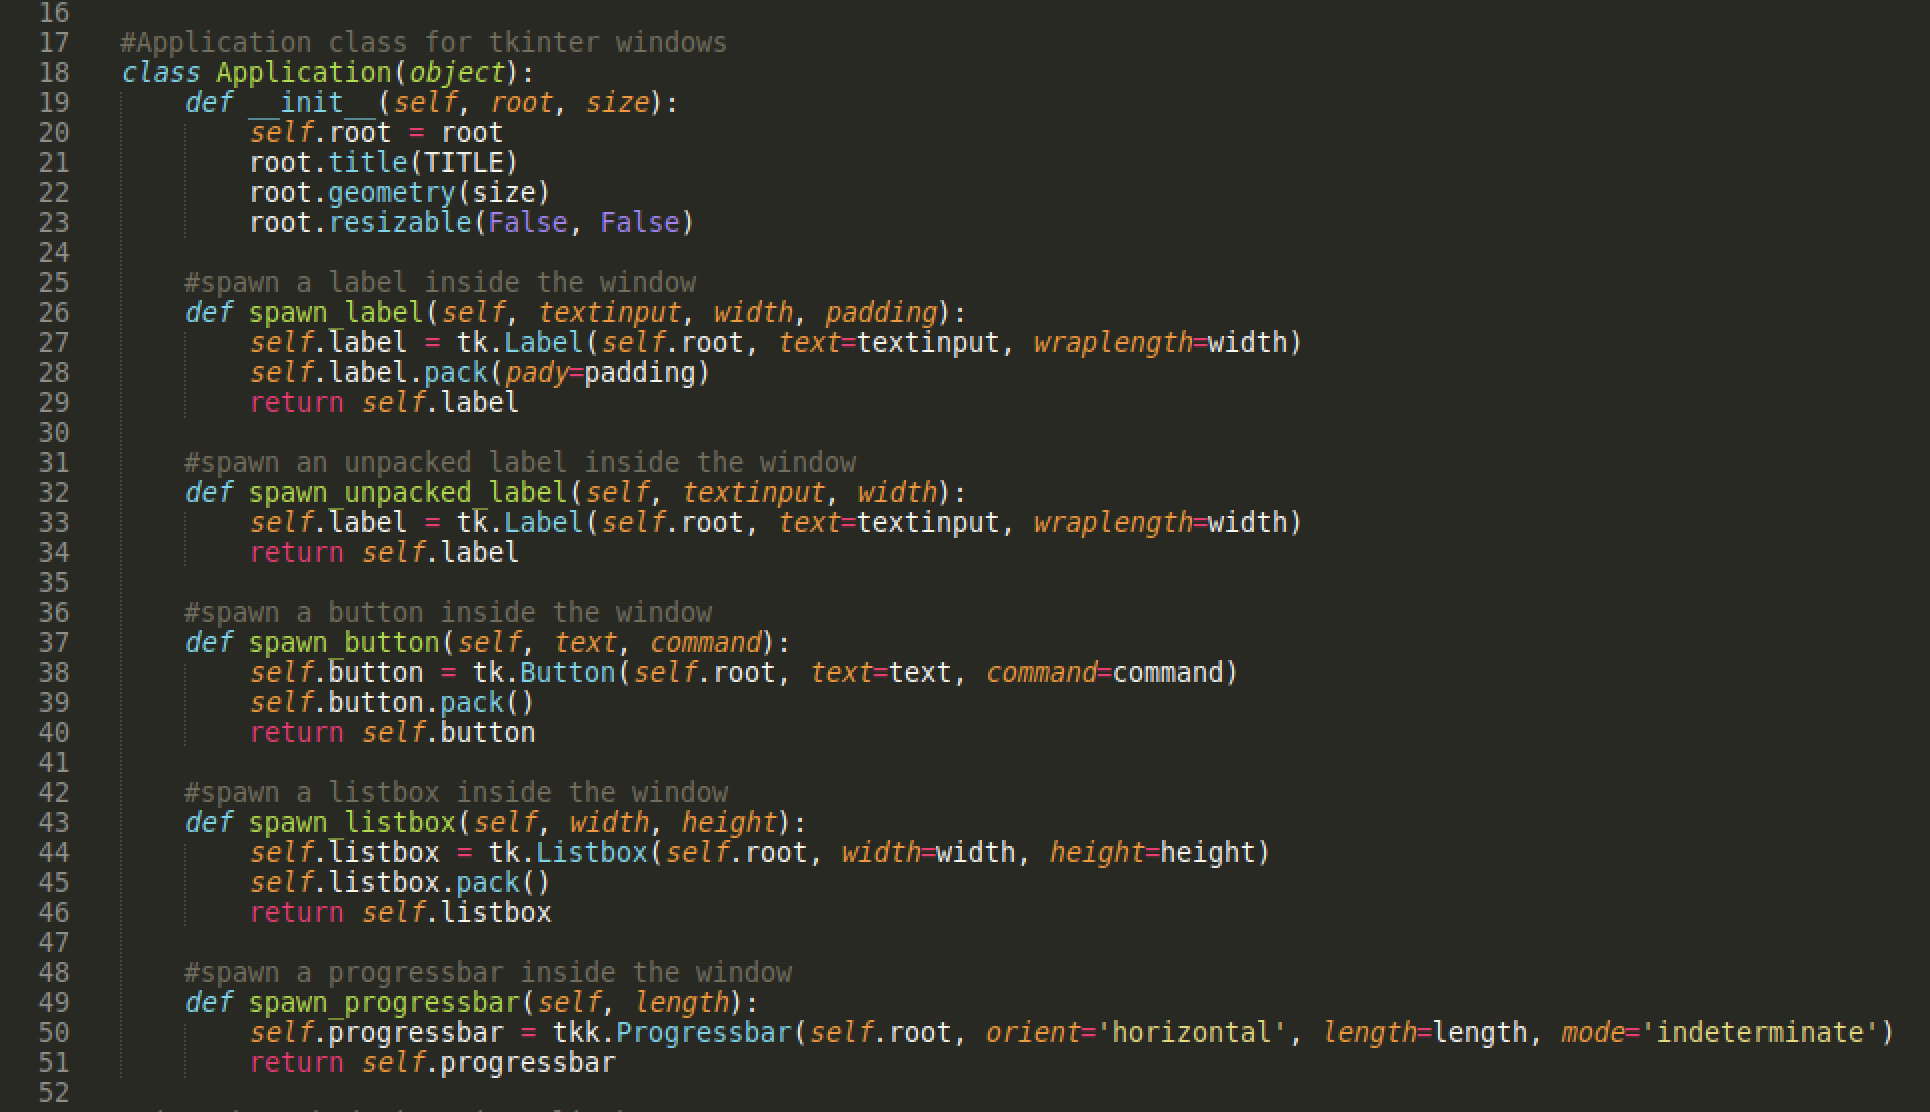
\includegraphics[height=9cm]{code_cutout_tkinter}
\caption{A sample of the Application class in rng\_test\_suite.py. This is used in each generated window to provide widgets such as labels, buttons, etc.}
\label{fig:code_cutout_tkinter}
\end{center}
\end{figure}

\begin{figure}[h!]
\begin{center}
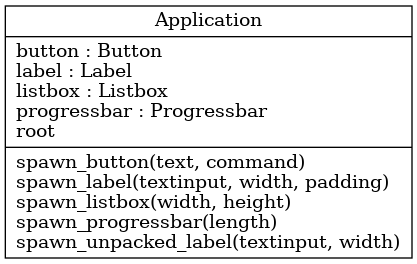
\includegraphics[height=4cm]{UMLclass}
\caption{A UML representation of the Application class and its components.}
\label{fig:UMLclass}
\end{center}
\end{figure}

\par{Now, using the Application class, I am generating a window where the user can list each device connected to the machine (be it physical or virtual). This window will use a listbox widget from the Tkinter Application class in order to list each item from \textit{/dev/*}.  If the user wishes to use a device in this program, it needs to be connected to /dev. It is stated in the program (for the convenience of the user) that it only lists devices from that machine environment listing.}

\par{As we want the program developed in this report, to implement the tests mentioned, from TestU01. The quality assurance of this, is important. The program should not bias the processing of the random output other than the time it takes to perform the tests. To ensure this, a couple of test runs will be performed on the /dev/urandom generator, a hardware random number generator and a known biased generator provided from TestU01. These generators will be sent through the program, and we will have a look at the testing speed, the outcome of the tests, and whether or not it provides the user with a feasible output that can be used for efficient testing of up to many devices over a shorter amount of time.}

\par{The implementation of the tests are done by installing TestU01 on the local system and adding some of its libraries to our system path. By adding the TestU01 testing libraries to our path, we are able to locally execute the tests in this program that has been developed. In Figure \ref{fig:code_cutout_SmallCrush} we can see an excerpt from the C file of the SmallCrush test suite. It takes an input file (which we will take a closer look at), runs the tests in the SmallCrush testing suite and outputs the results in standard output (stdout). The stdout is read by our main Python program which interprets whether or not it passes all the tests}

\begin{figure}[h!]
\begin{center}
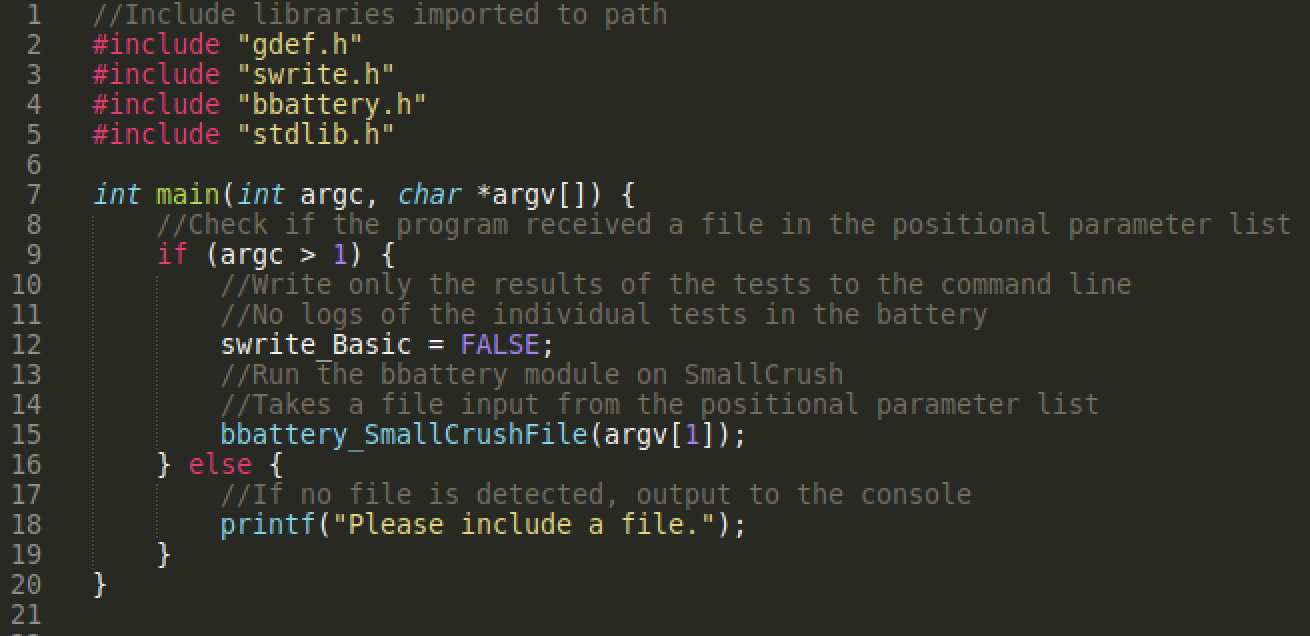
\includegraphics[height=8cm]{code_cutout_SmallCrush}
\caption{An excerpt from the C file SmallCrushTesting.c that runs the SmallCrush tests on a formatted RNG output}
\label{fig:code_cutout_SmallCrush}
\end{center}
\end{figure}

\par{As we can see, the C file implements some libraries that was important earlier through adding them to the environments path of our system. This is one of the benefits of the program that I made. It incorporates most of the manual process of testing through TestU01 inside the program structure. The Makefile that is supplied with this project builds most of the files necessary to run the Python program. However, one manual process that needs to be performed by the end-user at this point, is adding the libraries to the environment path. In the future, for another program that builds off the idea of a user-friendly testing suite to mitigate Random Number Generators with internal adversarial bias. Could be aware of this extra step in the TestU01 library and try to incorporate a way to make this an automatic process. Another potential improvement with the implementation of TestU01 and its libraries is to make a GUI program that has a Makefile attached to it. The Makefile is running before the testing process starts. Ensuring that all the necessary libraries are installed.}

\par{An important aspect of testing with the SmallCrush tests is the specifications provided by TestU01. As earlier mentioned, the SmallCrush tests needs a formatted output in order to run its tests against a RNG. To not bias the source, and remain the output as normalised as possible. A normalising function has been used within Python, before sending it to the actual Small Crush test suite. In Figure \ref{fig:code_cutout_ffb} we can see the flow of the converter.}

\par{It opens up the file (with raw RNG output) given from the positional parameter option in this python program. The file is read as a binary data file and converted to the representative and supported floating-point integers given in the specification of the test suite. As the floating-points needs to be in the set [0,1), we need to normalise the data between this set. Using one-dimensional linear interpolation through Numpy.interp(), the requested format can be achieved as seen in the method 'NormalizeData'. Here, once interpolated to our requested format between 0 and less than 1 in a floating-point representation, we apply a whitespace character between each float. This is printed to standard output and read by the main python program running in the background.}

\begin{figure}[h!]
\begin{center}
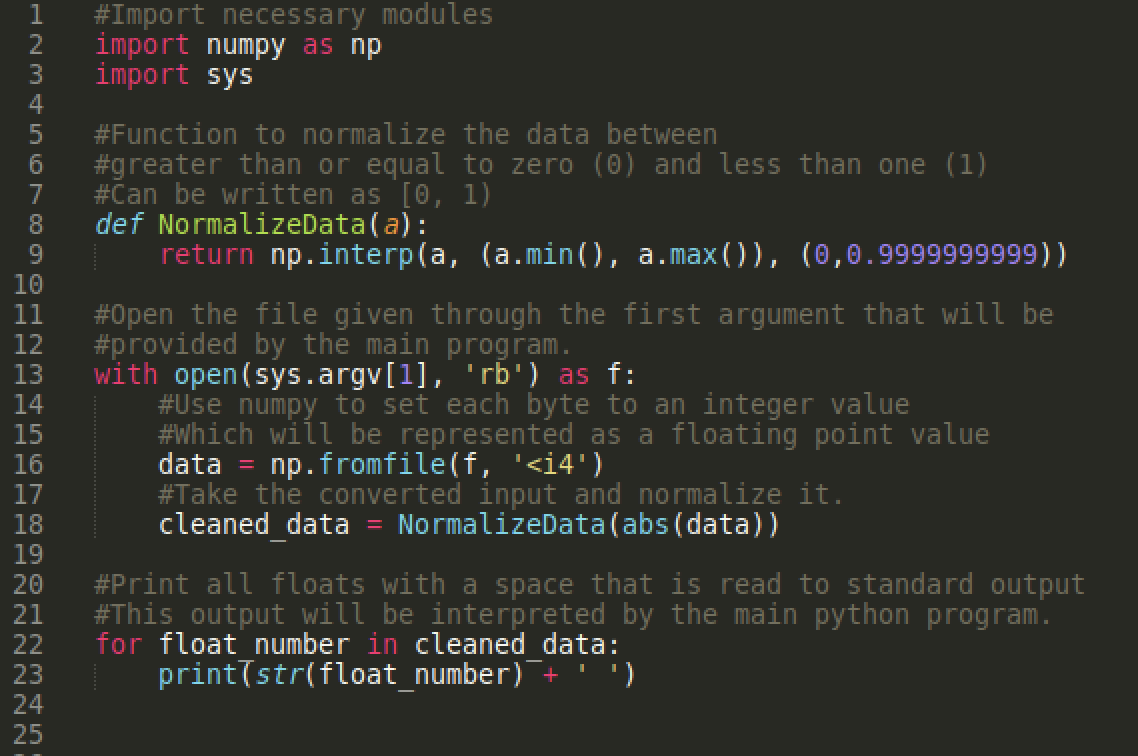
\includegraphics[height=8cm]{code_cutout_ffb}
\caption{The python file ffb.py that converts the raw output of the RNG and transforms it into SmallCrush suitable floating-point integers with a whitespace in between each float.}
\label{fig:code_cutout_ffb}
\end{center}
\end{figure}

\par{During the implementation of this external python file \textit{(ffb.py)}. Another approach was considered. Instead of having it as an external file, serving the exact same functions as a single method in my main python program. However, I found that if this program were to be further developed. Having separate files for formatting output could be a good idea for further implementations of different test suites, as appending new files for formatting to another specification could be done. So, to allow for further tests to simply be appended, the above method with an external file for specification formatting is used.}

\par{The FIPS testing does not need any formatted output, and takes the raw stream of characters generated by the RNG as input.}

\par{In the main python program \textit{rng\_test\_suite.py} the standard output from the FIPS testing and the SmallCrush testing is evaluated. Both of them writes to the end of the file if they successfully passed all the tests. We use this to locally evaluate the test results in the python program. As seen in Figure \ref{fig:code_cutout_run_tests} we have a method that is called upon the user requesting an analysis of a given RNG (through its system path). The method \textit{run\_tests\_on\_usb\_device()} takes 4 positional arguments. The first argument is the root of the current Tkinter window. The second is the path of the RNG. The third argument is the progressbar running in the background. Finally, the last argument is the text that displays in what stage of the testing phases the program is in. E.g. the test is formatting output to a specified format.}

\begin{figure}[h!]
\begin{center}
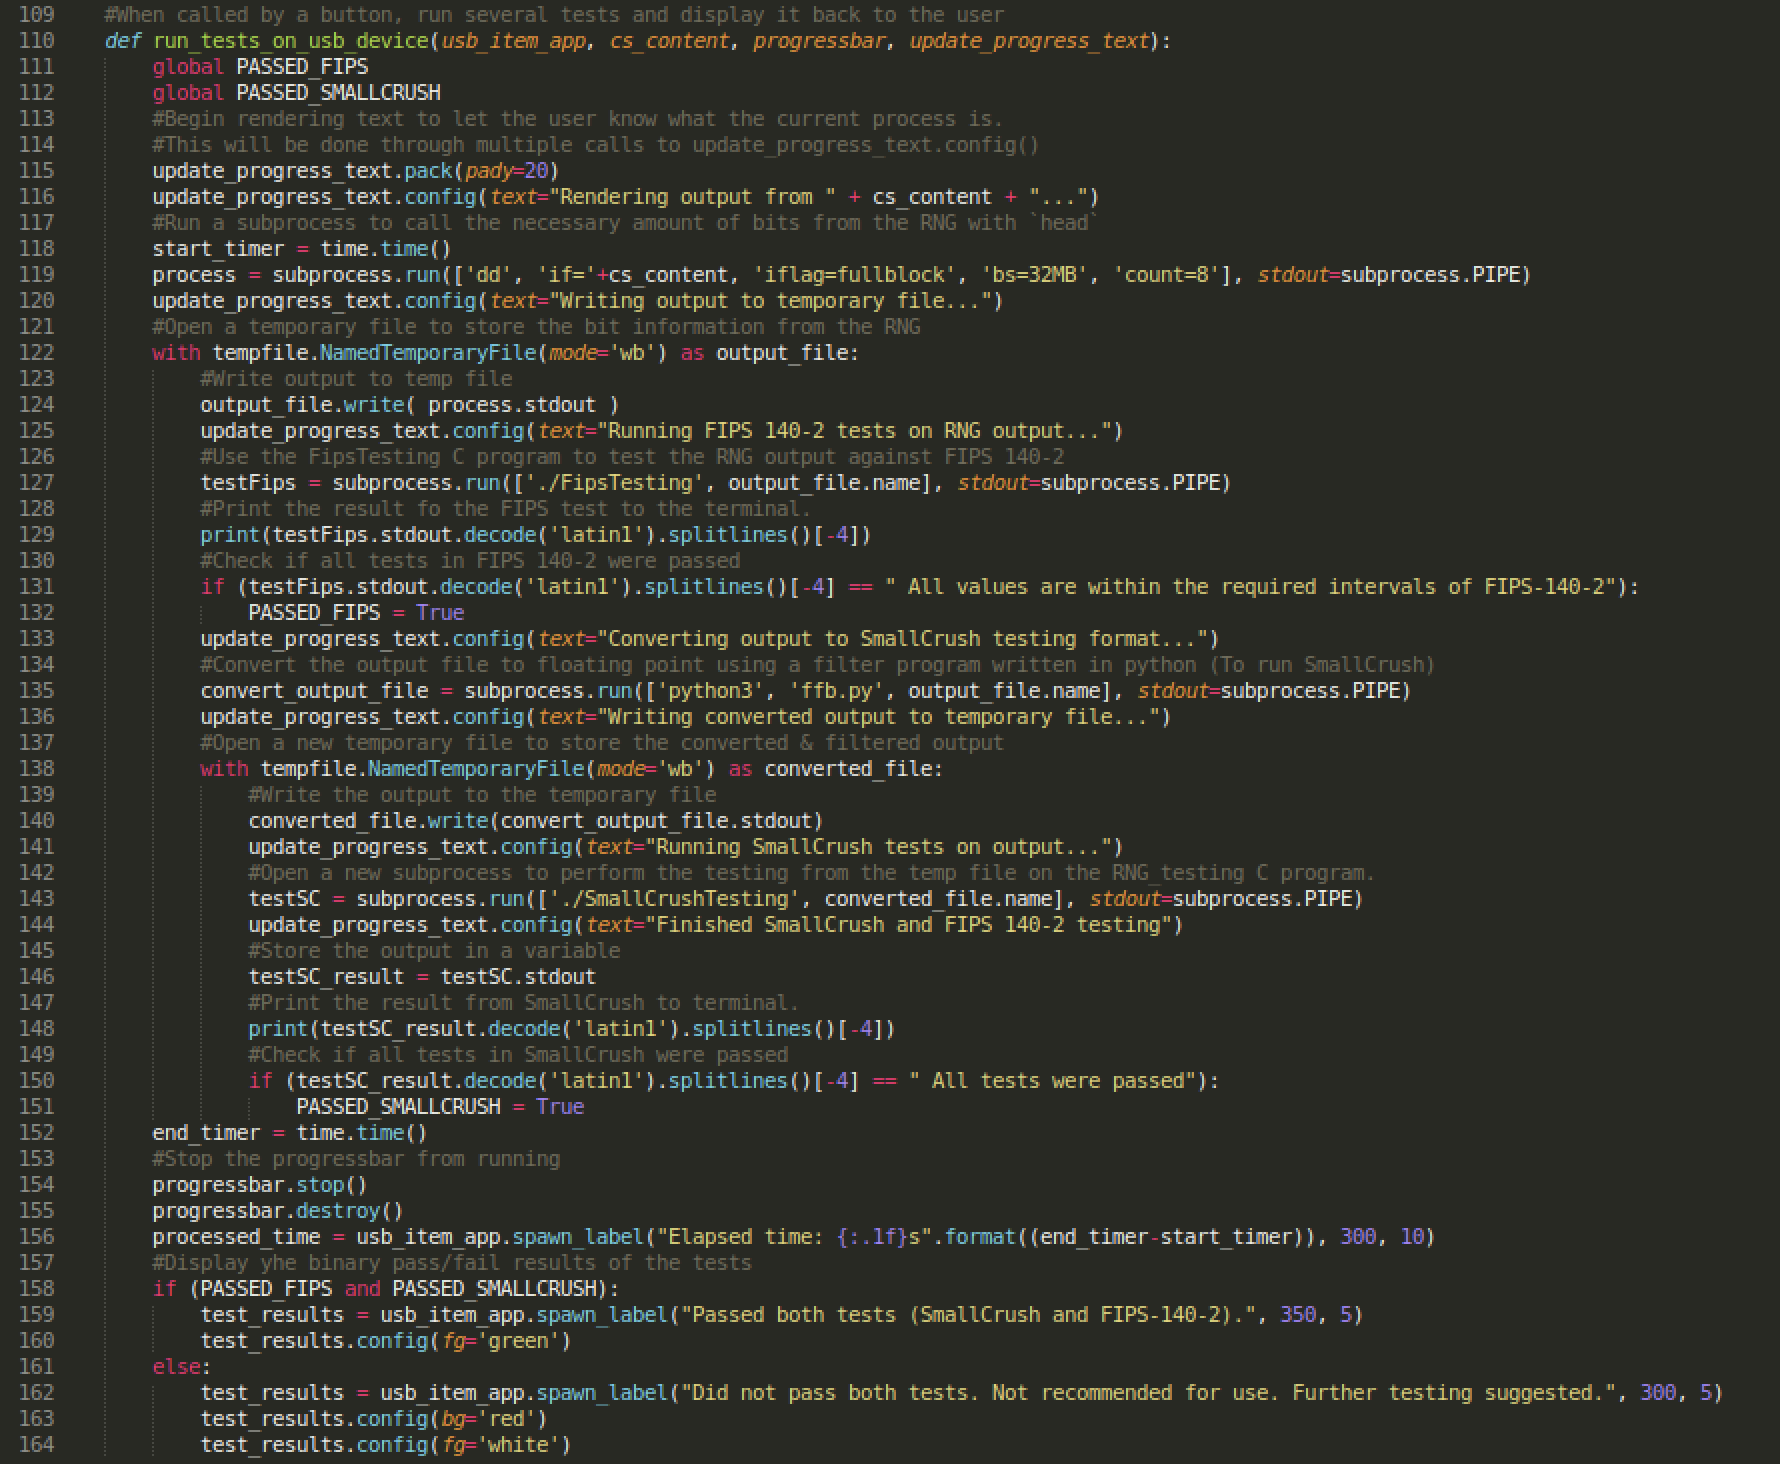
\includegraphics[height=12cm]{code_cutout_run_tests}
\caption{The method run\_tests\_on\_usb\_device() in the main python program}
\label{fig:code_cutout_run_tests}
\end{center}
\end{figure}

\par{We use the path of the RNG to run a subprocess which uses the command line function 'dd' in order to retrieve the sufficient amount of bits from the RNG. Previously 'head' was used, but I found that the 'dd' command lets me use the 'iflag' option to make it wait for all the bits to be provided before terminating, whereas 'head' may terminate without providing all the bits that was requested. In this program I request 32*8MB=256MB of output data from the RNG. SmallCrush requires just around 51320000 random numbers in order to successfully run. Therefore providing it with a large amount that is guaranteed to be over the requested number helps us ensure that the program will not fail.}

\par{The program writes the output into a temporary file stored locally on the system. My FIPS 140-2 test C-program runs a subprocess that evaluates whether or not the output passes the test suite. If it passes, a global variable is set to True. The file is read as a binary file in order to be processed correctly by the C testing program.}

\par{After this, the program opens a new subprocess that runs the previously discussed ffb.py file with the output that is stored in the temp file. This is saved into a variable that is later used in a new temporary file that stores the formatted data from ffb.py. Using the formatted output, it opens yet another subprocess that performs the SmallCrush tests through the compiled SmallCrushTesting.c file. The output of this test is written to standard output, and read by this main python program. The test results are stored in a variable and read by the program, which checks whether or not it can identify the string that shows whether or not all the tests passed. If the tests are seemingly passing, the global variable for SmallCrush testing is set to True.}

\par{in the end of the main python program, we run a quick check to see whether or not both the FIPS and SmallCrush tests passed. If they both passed, a green label with information that it successfully passed both tests is displayed. If the test suites failed or one of them failed, a red label is shown, which tells the user that it is not recommended for use by this program. Further testing is suggested. As this is a proposal for more user-friendly programs, another program could implement an output label that instructs the user of what tests failed and maybe a bar which shows the total percentage of tests that failed. This could help the user draw a better picture of whether or not stringent adversarial bias may have been implemented in the RNG.}

\par{As seen in Figure \ref{fig:code_output_run_tests}, the method takes two positional parameters as arguments at the foot of the method. The progressbar and the text that updates based on the progress made in the program. These two methods are a User Experience design feature. It lets the user know whether or not the program is actually running, and where it currently is in the testing process. The progressbar is running as a separate thread in order to not disrupt the thread running the actual tests. The updated text is providing updates to the user while running different consequential steps from the test regime. A timer is also calculating the time it takes from the tests are started, until it finishes. This helps the user understand the progress made by the program in real-time.}

\chapter*{Testing and Results}
\addcontentsline{toc}{chapter}{Testing and Results}

\par{The program implements two statistical test suites. One known for not being able to detect some structural bias (FIPS 140-2) and one that is considered a better collection of tests by TestU01 (SmallCrush). Having these two suites, it can help us try to detect bias in generators we know have bias implemented in them. TestU01 incorporates such a generator which we can use to test our set of test suites.}

\par{In the supply chain of Random Number Generators, we have threat vectors that could potentially enter. We have discussed structural bias as one of the most damaging, as it can result in a RNGs output to be predictable to an adversary by exploiting the output stream of the RNG. In order to test whether or not the program developed in this project correctly implements the TestU01 tests SmallCrush and FIPS 140-2, three generators will be performed on the test suites through the program.}

\par{TestU01 contains a library known as unif01gen, where we can create a bias in the output stream of a generator. The original stream will be poisoned with constant density through some set values of a probability over an interval \textit{[0, a]}\cite{Ecuyer:2007}. Where the probability  p and a is set to different values to affect the RNG output strictly. We will use this biased generator over the output stream of one RNG with a different value for p and a for each run. This will be a biased output from the TectroLabs TL200. We will use the raw output from the TRNG TectroLabs TL200 as well for testing. Finally, testing the outcome of /dev/urandom from our local machine will also be performed. /dev/urandom uses the same entropy pool as /dev/random, and /dev/random being a blocking generator, we will prioritise urandom for these tests. 4 tests will be performed on each different RNG to check whether or not bias is detected.}

\par{A file BiasedGen.c has been compiled into BiasedGen to run a biased generator over the output of another generator. This can be used for any generator attached to the /dev/ environment. The file it not used in the actual program, but was used for testing.}

\begin{tabular}{ |p{3cm}||p{1.5cm}|p{1.5cm}|p{1.5cm}|p{1.5cm}|p{2cm}| }
 \hline
 \multicolumn{6}{|c|}{\textbf{\textit{Test results}}} \\
 \hline
 \textbf{RNG}& \textbf{Test 1} & \textbf{Test 2} & \textbf{Test 3} & \textbf{Test 4} & \textbf{Avg time:}\\
 \hline
 /dev/urandom  & Passed & Passed & Passed & Passed & 127.7s\\ 
 \hline
 TectroLabs TL200 & Passed & Passed & Passed & Passed & 98.3s\\
 \hline
 Biased TL200 & Failed & Failed & Failed & Failed & 90.4s\\
 \hline
\end{tabular}

\par{When running a test, we will see either a pass or a fail window. The output of the stdout will be more detailed, for those who may want to look at the individual tests this will be available in the console. As we can see from Figure \ref{fig:program_cutout_fail} and \ref{fig:program_cutout_pass}, the graphical outcome of the results is very simple for the user to quickly identify whether or not the generator is recommended by the program. The generator will be recommended if all tests pass.}

\begin{figure}[h!]
\begin{center}
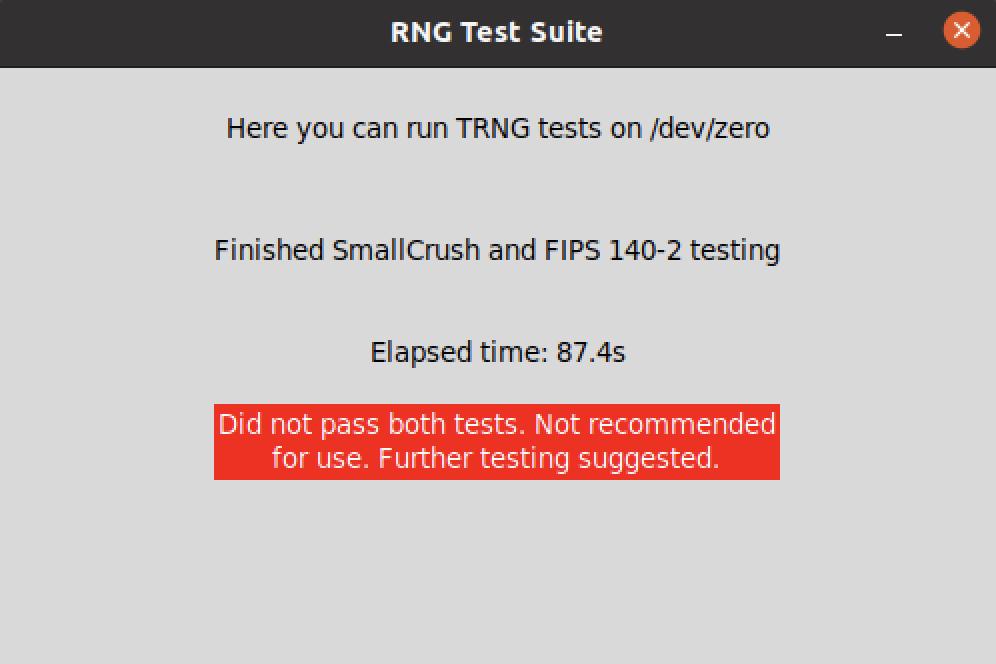
\includegraphics[height=8cm]{program_cutout_fail}
\caption{A sample program output of /dev/zero failing. The /dev/zero is expected to fail all tests heavily as it just outputs zeroes.}
\label{fig:program_cutout_fail}
\end{center}
\end{figure}

\begin{figure}[h!]
\begin{center}
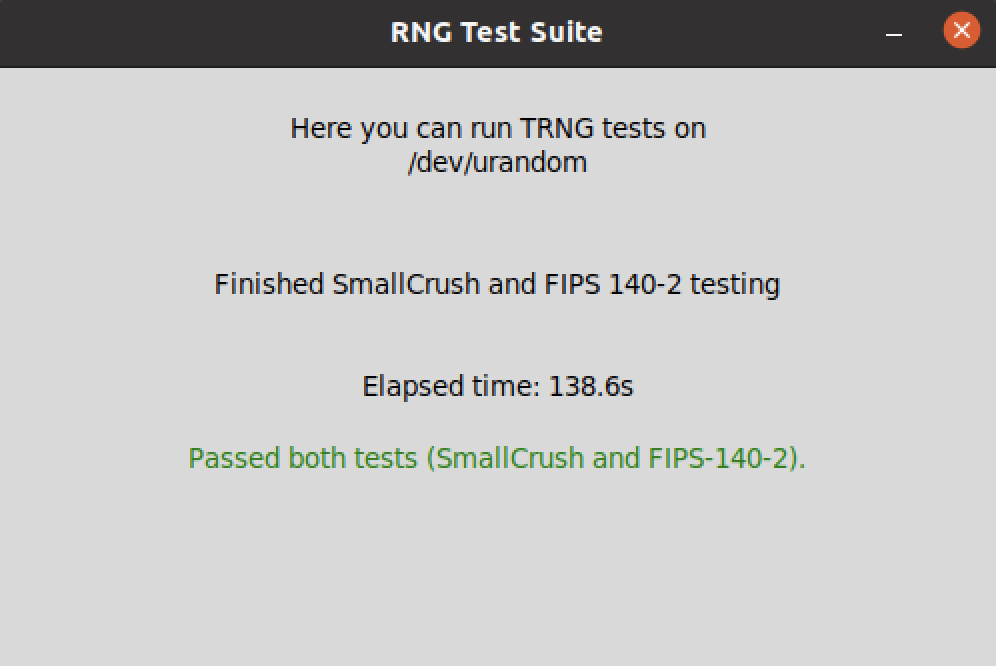
\includegraphics[height=8cm]{program_cutout_pass}
\caption{A sample program output of /dev/urandom passing the test suites.}
\label{fig:program_cutout_pass}
\end{center}
\end{figure}

\par{As we can see from these results, our set of statistical test suites in the program are able to detect the bias that was implemented in our TRNG output stream. This is not conclusive evidence as to whether or not the program that was developed is able to detect all bias, but it can be used as a proposal for further programs to be developed. The tests shows that currently, SmallCrush is able to detect the bias it was given from the generated bias (constant density). However, when the same bias was applied to the FIPS testing of the generator. It did pass most of the tests each time, except three individual tests in total for all test runs.}

\par{If we had implemented less bias (as this was a stringent method of creating bias in the generators), we could have seen different results. One interesting outcome would be that the FIPS tests pass and the SmallCrush tests fails drastically, as it did in this example. We can see that for this test regime that was performed, the FIPS tests were able to actually detect the bias. For more discrete bias, it may have been a different outcome.}

\par{Having an easy way of testing RNGs can help mitigate some of the risks found in the supply chain entering a system. Some lightweight statistical tests, like SmallCrush, may very well be able to detect some of this structural bias. However, more stringent and thorough test suites should be implemented to properly search for more discrete bias. Crush and BigCrush are examples of such tests, even though their testing times may be drastically higher than the SmallCrush test. As discussed previously, having these as optional tests could be an alternative.}

\chapter*{Professional Issues}
\addcontentsline{toc}{chapter}{Professional Issues}
\par{During the development of the program and researching Random Number Generators through professional research papers, care had to be taken in order to prevent misleading citations in this report. Having a strong and lengthy reference list, obtaining control over the citations is important. The sources used for this paper has been carefully picked and evaluated before use. Where appropriate, the authors have been acknowledged. No author has been referenced in the bibliography, without being directly cited for its use in this report.}

\par{Following the British Computing Society (BCS) Code of Conduct, I have taken careful notes of what should be included in this paper, in terms of references. Also, as the BCS states \cite{BCS:2020}, ``The BCS Code of Conduct serves as a unique and powerful endorsement of your integrity and as a code of ethics for IT professionals.''. Using the Code of Conduct as a guideline for this report has helped keeping the integrity of both my work and the work of those whose cited.}

\par{Following the Code of Good Practice for Research \cite{RHCGPR:2020} by my university institution; Royal Holloway. I have strived to write this paper on the background of this. Especially taking note of the General Expectations of Researchers section:}

\begin{enumerate}
\item{To produce research and research outputs that meet international standards of excellence}
\item{To seek appropriate funding to support research, impact and knowledge exchange activity}
\item{To create transformational impacts for individuals, society, and the environment, by collaborating
externally and through knowledge exchange}
\item{To contribute to an excellent research culture by engaging in the wider research activities of their
department and institution}
\item{To provide research leadership}
\item{To comply with College and external research related policies, codes and concordats}
\end{enumerate}

\par{In this report, a relevant issue has been the software design process. Where different design ideas had to be taken into consideration. For the main python program that was developed. I decided to go with an Application class for the Tkinter windows. This was a design decision that was taken on background of how I knew that the windows would spawn. I first started out without the Application class, but just using the inbuilt methods of Tkinter raw. This led me to actively having to pack() each window widget. This was both tedious and the code ended up harder to read as a result of this. I changed my program to incorporate the Application class after this. A UML for this specific class (which ended up to be my only class) can be found in Figure \ref{fig:UMLclass}}
	
%%%%%%%%%%%%%%%%%%%%%%
%%% Reflective Statement
\chapter*{Reflective Statement from Interim Review}
\addcontentsline{toc}{chapter}{Reflective Statement}

\par{Up until this point in the report, handing in the interim review, I have been through research in the broad topic of Random Number Generators. To narrow my research down and to answer my dissertation title, I have been looking into the supply chain of Hardware Random Number Generators. I have also been looking into the aspects of supply chain attacks against critical security infrastructure of HRNGs.}

\par{During the last months I have been writing on two different and essential reports for this project. A report on HRNGs, where I try to identify some of the main characteristics of a HRNG and how it is different from a PRNG. The second report was on supply chain attacks and how we can mitigate them. The conclusions of these reports are open and no answer is given as I find that to be out of scope for this project. I focused entirely on the reading list and finding already conducted experiments.}

\par{At this point I have written some test software in C to try to better understand the underlying tests of statistical test suites. However, as of now, writing programs has not been a priority. I have stated some of my intents for the next iteration of my report in the methodology chapter. I hope to write some more code to understand the test suites even better, and to maybe implement graphs developed in MatLab into my report.}

\par{The graphs or illustrations generated from MatLab would be aimed at showing statistical analysis of test results from my programs.}

\par{Progressing from this stage, I would like to see if a proposal of a decontamination protocol for TRNGs leaving the supply chain could be a good idea. If not, why? And also perform further research on the supply chain to better understand if a decontamination protocol is necessary.}

\section*{Future aims}
\addcontentsline{toc}{section}{Future aims}

\par{In the subsequent report after the interim review I aim to have conducted some statistical tests, analysed them and produced meaningful graphs/illustrations to showcase the results.}

\par{To be able to conduct these experiments I will need to analyse the content of other researchers and most likely cite some of their code and findings. What procedures and methodology they have been using may be of interest for this project. As I will not try to fully recreate any experiments or make any attempts at conducting new experiments as that will be out of scope for this project.}

\par{A great focus area of the next iteration of the report will be to extensively document my code and statistical tests. This will be compassed through UML diagrams and commenting the code. It should not be trivial to perform adequate Test Driven Development on the Python and C code I will be writing which will be simple implementations of already functioning tests, described in their respective test suite documentation}

\par{As some researchers already have found, some tests are not suited to be hardware implemented. It would be interesting to have a deeper look into these particular tests and see why they only are suitable for software implementations. The end goal of this particular dilemma being to find which tests are suitable and what their characteristics are.}

\par{Eventually, having a look at the idea of introducing a decontamination protocol or another remediation protocol as a standard for TRNGs when they are handed over to the end-user.}

\par{To analyse this I will do more research on earlier attempts at mitigating effects of supply chain attacks in the past. There might even be some published work that has come to a conclusion. Either way, I will not be conducting my own protocol implementation tests as that would be out of this projects scope, but I might gather all the research and then conclude with my findings.}

\section*{Diary entries}
\addcontentsline{toc}{section}{Diary entries}

\par{Each week I have logged all of my diary entries to the departmental diary webpage\footnote{\url{https://pd.cs.rhul.ac.uk/2020-21/}}. A quick summary of the sum of the entries listed below.}

\begin{itemize}
\item{A bi-weekly meeting with my supervisor to discuss the progress on the reports and the interim review.}
\item{Logged my status on the report writing each week.}
\item{Logged my status on reading required research for each report and for the interim review each week.}
\item{Logged any findings which may have caused particular interest.}
\item{Logged current concerns regarding the project as they appeared.}
\end{itemize}


%%%%%%%%%%%%%%%%%%%%%%
%%% Bibliography
\newpage
\addcontentsline{toc}{chapter}{Bibliography}

\bibliographystyle{plain}
\bibliography{main}

\label{endpage}

%%%%%%%%%%%%%%%%%%%%%%
%%% Appendix A
\chapter*{Appendix A}
\label{appendixa}
\addcontentsline{toc}{chapter}{Appendix A}

\subsection*{Locating the code}
\par{The code written so far in this project is located in the SVN repository.}
\par{To find all written code, locate /zfac134/final\_year\_project/trunk/code}

\subsection*{Installing and building necessary libraries}

\textbf{NOTE:} For this project, a Makefile has been provided to do most of this automatically. However, some of the steps, like building the environment libraries for TestU01 has to be done manually.

This appendix is made in order to manually go through each installation step in case it is needed.

\subsubsection*{Prerequisities}
\begin{itemize}
\item{git and gcc installed on the target system}
\end{itemize}

\subsubsection*{Installing TestU01}
1. Run this to clone their GitHub repository
\begin{lstlisting}
    # git clone https://github.com/umontreal-simul/TestU01-2009.git
\end{lstlisting}
2. In order to compile the programs, the 3 following paths must be added to the environment variables:
\begin{lstlisting}[language=bash]
    LD_LIBRARY_PATH    <install directory>/mylib
    LIBRARY_PATH       <install directory>/mylib
    C_INCLUDE_PATH     <install directory>/include
\end{lstlisting}

If this is compiled using a UNIX environment, we will perform the following commands in the Bourne shell to add them to the environment variables:

\begin{lstlisting}[language=bash]
    export LD_LIBRARY_PATH=<install directory>/mylib:{LD_LIBRARY_PATH}
    export LIBRARY_PATH=<install directory>/mylib:{LIBRARY_PATH}
    export C_INCLUDE_PATH=<install directory>/include:{C_INCLUDE_PATH}
\end{lstlisting}

Simply replace $<$install directory$>$ with the directory path of the git clone. \textit{Note that on some UNIX systems like MacOS, mylib is used instead of lib in LD\_LIBRARY\_PATH and LIBRARY\_PATH.}

3. In order to compile programs, as stated by the instalment guide:
\begin{lstlisting}[language=bash]
    gcc <program path> -ltestu01 -lprobdist -lmylib -lm
\end{lstlisting}

\subsubsection*{TL200: Building and loading tlrandom}
\par{Running the Makefile will build the necessary packages and add the TL200 to the /dev/ compartment of your Linux OS. However, if a manual process is preferred. It is provided here.}

\par{From TectroLabs's Github page, please proceed with cloning the following repository. \textit{git clone https://github.com/tectrolabs/tl200} This repository contains the necessary files in order to add TL200 to our /dev path. Proceed by unpacking the newest directory from TL200. This directory will include a number of different OS compatible subdirectories. For our purposes, the Linux-64 folder is the one we will be using.}

\par{In this folder, navigate to /getrnd and perform a \textit{sudo make} command. This will provide the necessary tools in order to run the TL 200 on our system. 
NOTE: If you have a TL200 that is not configured correctly for Linux. Please follow the instructions in this subdirectory by performing the following command to get more info: \textit{./getrnd}}

\par{Now proceed by heading into the directory ../tlrandom and run a \textit{make} command here as well. This will generate quite a few additional files in our repository. Now, to finish the installation of TL200 in our /dev path. Please run \textit{sudo chmod +x} on the /ins-tlrandom.sh to make it executable for us as a user. Then proceed with \textit{./ins-tlrandom.sh}}

\par{The TL200 device should now be able to be read from /dev. Check this by performing the following command: \textit{sudo head -c 100 /dev/tlrandom}. This should produce 100 bits of random output from the TL200 device.}

\par{If you had problems following the instructions, please resort to the guidelines and documentations asserted by TectroLabs. There should be a README file located inside the linux-64 directory of this repository.}


\end{document}

\end{article}
